\documentclass{beamer}
%% \documentclass[draft]{beamer} %% draft version

%% restrict generation of slides
%% \includeonlyframes{oligoarray,probesyn}

\mode<presentation>
{
  \usetheme{Bielefeld}
  \setbeamercovered{transparent}
}

\usepackage[english]{babel}
\usepackage[latin1]{inputenc}
\usepackage{graphicx}

\usepackage{lmodern}
\usepackage[T1]{fontenc}

\newcommand{\ignore}[1]{}

\title[WABI 2006 - Improving Microarray Layout: Pivot Partitioning] % (optional, use only with long paper titles)
{Improving the Layout of Oligonucleotide Microarrays: Pivot Partitioning}

%% \subtitle
%% {Include Only If Paper Has a Subtitle}

\author[S.~A.~de~Carvalho~Jr. (Universit\"at Bielefeld)] % (optional, use only with lots of authors)
{S\'ergio A. de Carvalho Jr.\inst{1,}\inst{2}\inst{,3} \and Sven Rahmann\inst{1,}\inst{2}}
% - Give the names in the same order as the appear in the paper.
% - Use the \inst{?} command only if the authors have different
%   affiliation.

\institute[Universit\"{a}t Bielefeld] % (optional, but mostly needed)
{
\inst{1}%
Algorithms and Statistics for Systems Biology, Genome Informatics,\\
Technische Fakult\"at, Universit\"at Bielefeld, Germany
\and
\inst{2}%
International NRW Graduate School in Bioinformatics and Genome Research
\and
\inst{3}%
Graduiertenkolleg Bioinformatik
}
% - Use the \inst command only if there are several affiliations.
% - Keep it simple, no one is interested in your street address.

\date[WABI 2006] % (optional, should be abbreviation of conference name)
{Workshop on Algorithms in Bioinformatics, 2006}
% - Either use conference name or its abbreviation.
% - Not really informative to the audience, more for people (including
%   yourself) who are reading the slides online

% \subject{Theoretical Computer Science}
% This is only inserted into the PDF information catalog. Can be left
% out. 

% If you have a file called "university-logo-filename.xxx", where xxx
% is a graphic format that can be processed by latex or pdflatex,
% resp., then you can add a logo as follows:

% \pgfdeclareimage[height=0.5cm]{university-logo}{university-logo-filename}
% \logo{\pgfuseimage{university-logo}}

% Delete this, if you do not want the table of contents to pop up at
% the beginning of each subsection:
\AtBeginSubsection[]
{
  \begin{frame}<beamer>
    \frametitle{Outline}
    \tableofcontents[currentsection,hideallsubsections]
  \end{frame}
}

% If you wish to uncover everything in a step-wise fashion, uncomment
% the following command: 
%\beamerdefaultoverlayspecification{<+->}


\begin{document}

%%%%%%%%%%%%%%%%%%%%%%%%%%%%%%%%%%%%%%%%%%%%%%%%%%%%%%%%%%%%%%%%%%%%%%%%%%%%%%%%
\frame[plain]{

  \vspace*{0.4cm}
  \centerline{
    
\includegraphics[height=1.3cm]{pics/aggi_logo.png}
    \hspace*{0.6cm}
    
\includegraphics[height=1.3cm]{pics/gsbg_logo.png}
  }
  
  \titlepage
}

%%%%%%%%%%%%%%%%%%%%%%%%%%%%%%%%%%%%%%%%%%%%%%%%%%%%%%%%%%%%%%%%%%%%%%%%%%%%%%%%
\frame{\frametitle{Outline}

  \tableofcontents[hideallsubsections]

}

%% *****************************************************************************
\section[Introduction]{Introduction to Microarray Layout}
\subsection{Dummy}
%% *****************************************************************************

%%%%%%%%%%%%%%%%%%%%%%%%%%%%%%%%%%%%%%%%%%%%%%%%%%%%%%%%%%%%%%%%%%%%%%%%%%%%%%%%
\frame[label=oligoarray]{\frametitle{High-Density Oligonucleotide Microarrays}

  \centerline{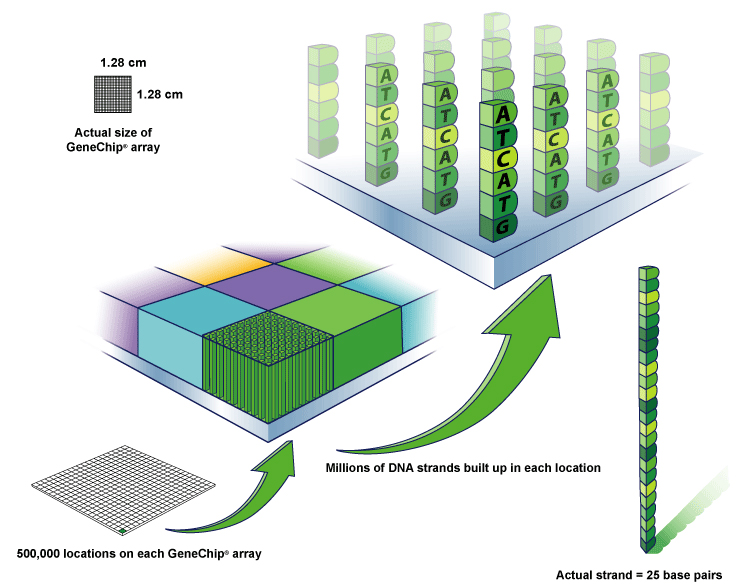
\includegraphics[height=0.9\textheight]{pics/oligoarray.jpg}}
  \vspace*{-0.5cm}
  \centerline{\tiny{Source: Affymetrix, Inc.}}

}

%%%%%%%%%%%%%%%%%%%%%%%%%%%%%%%%%%%%%%%%%%%%%%%%%%%%%%%%%%%%%%%%%%%%%%%%%%%%%%%%
\frame[label=probesyn]{\frametitle{Probe Synthesis with Photolitographic Masks}

  \vspace*{-0.5cm}
  \flushright{\tiny{Source: Affymetrix, Inc.}}
  \centerline{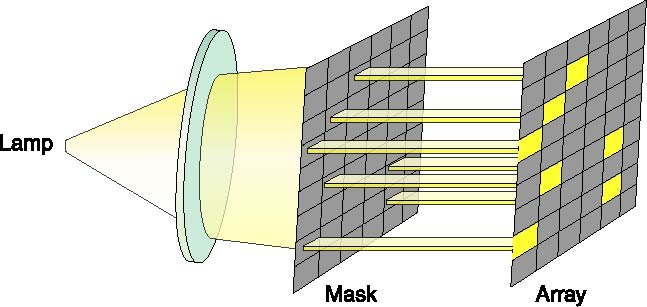
\includegraphics[height=0.5\textheight]{pics/photolithography.jpg}}  

  \begin{itemize}
    \item Probes are synthesized on the chip in a \alert{series of steps}
    \item Each step \alert{appends a particular nucleotide} to selected regions
    \item Selection occurs by exposure to light directed by a \alert{mask}
  \end{itemize}
}

%%%%%%%%%%%%%%%%%%%%%%%%%%%%%%%%%%%%%%%%%%%%%%%%%%%%%%%%%%%%%%%%%%%%%%%%%%%%%%%%
\frame[label=embed]{\frametitle{Deposition Sequence and Probe Embeddings}

  \begin{overprint}
  \onslide<+>
    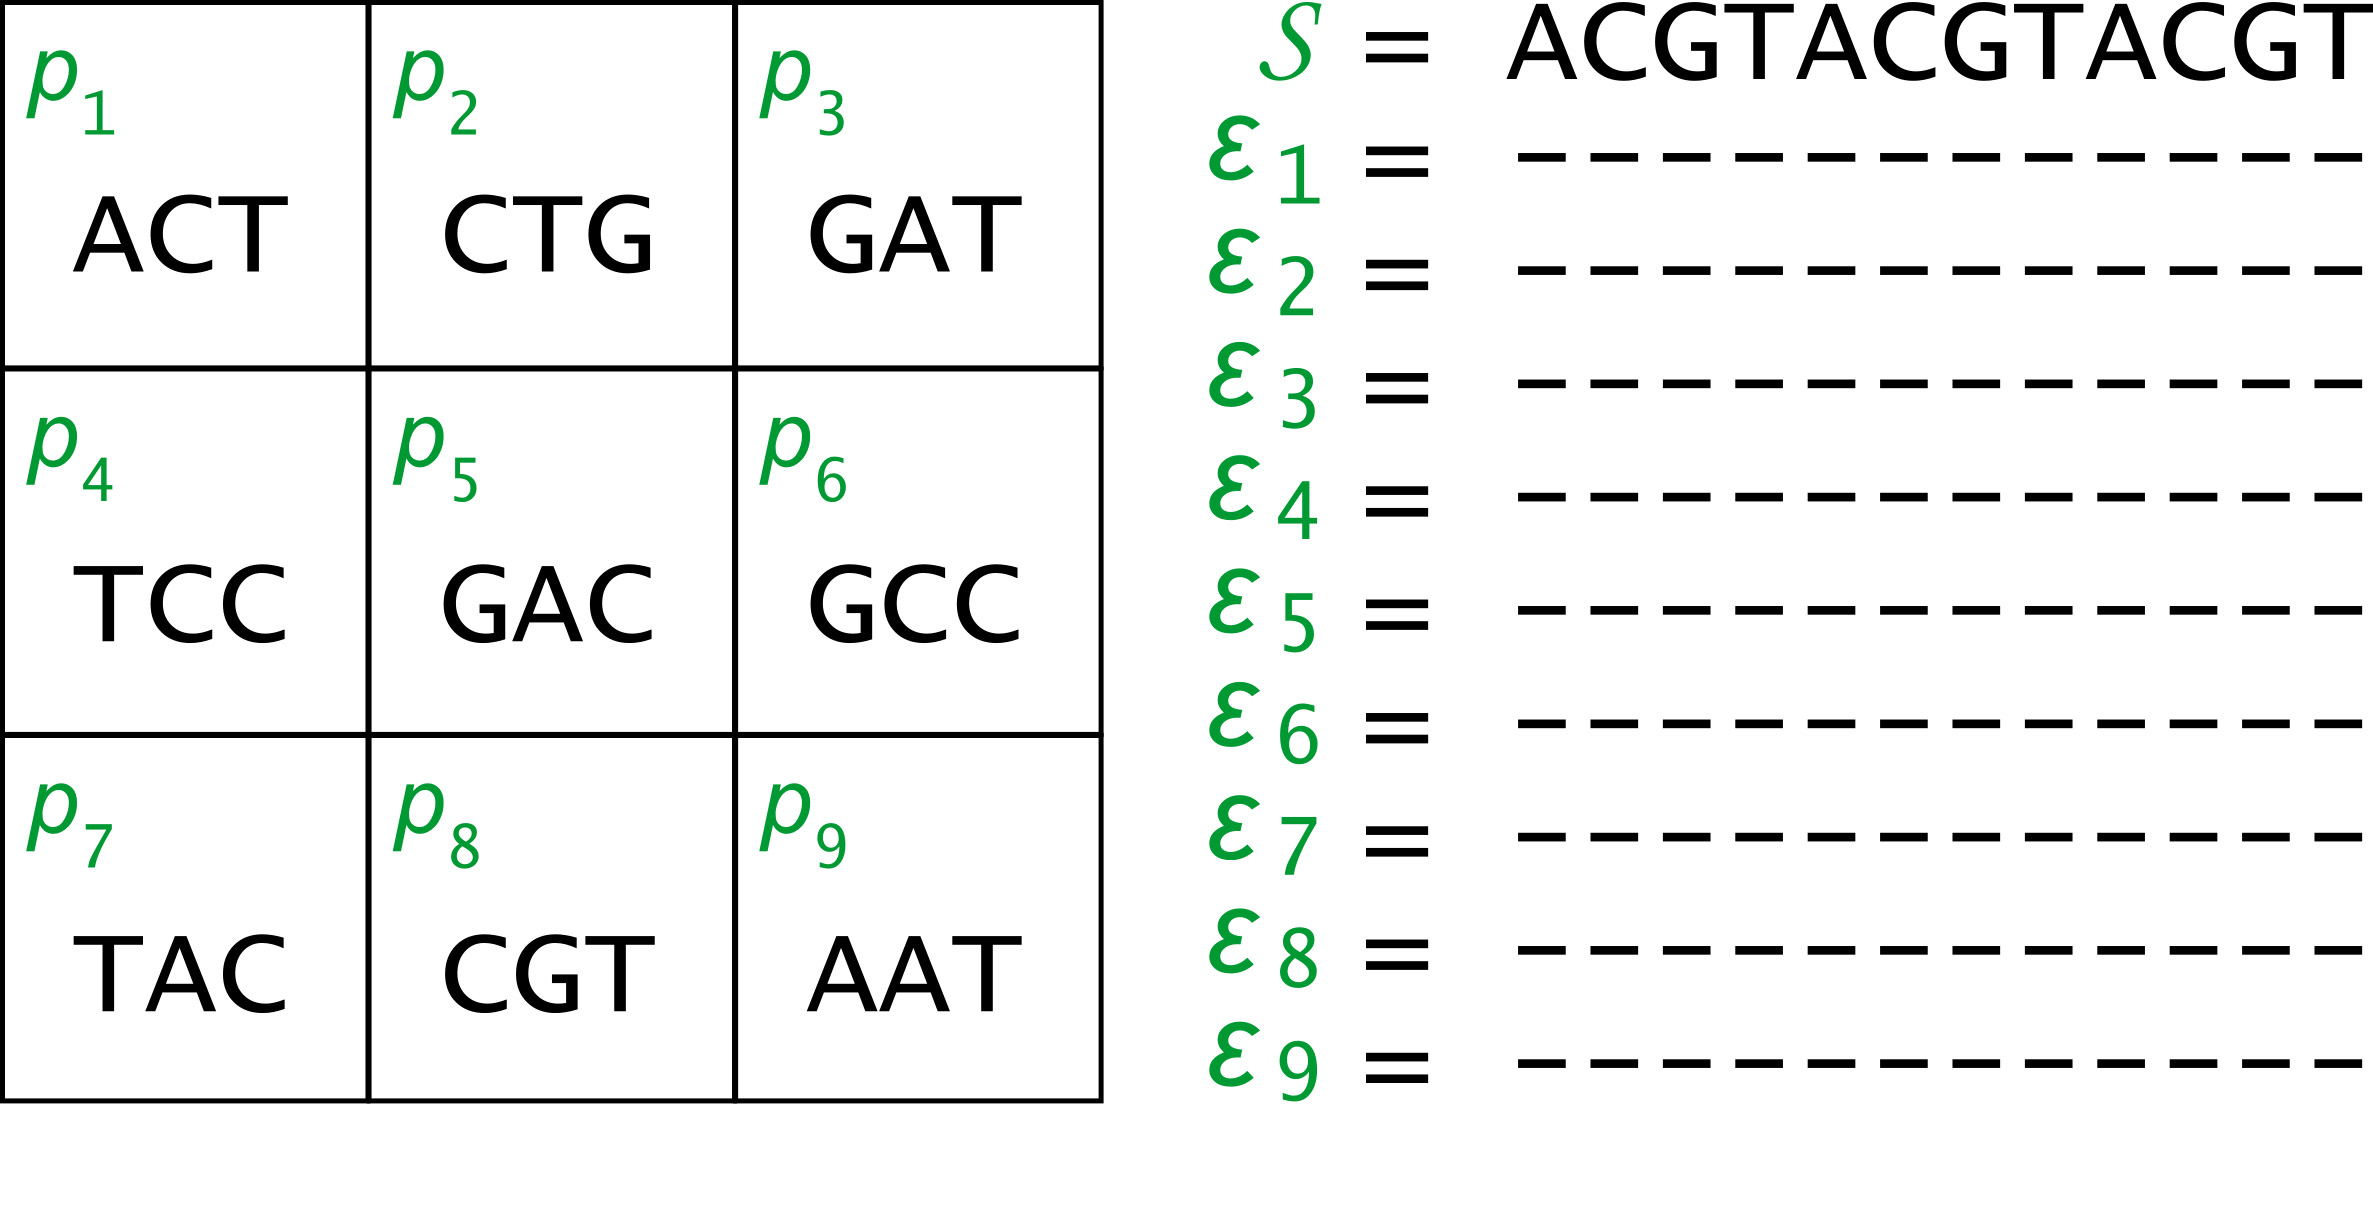
\includegraphics[width=\textwidth]{masks/chip.jpg}
  \onslide<+>
    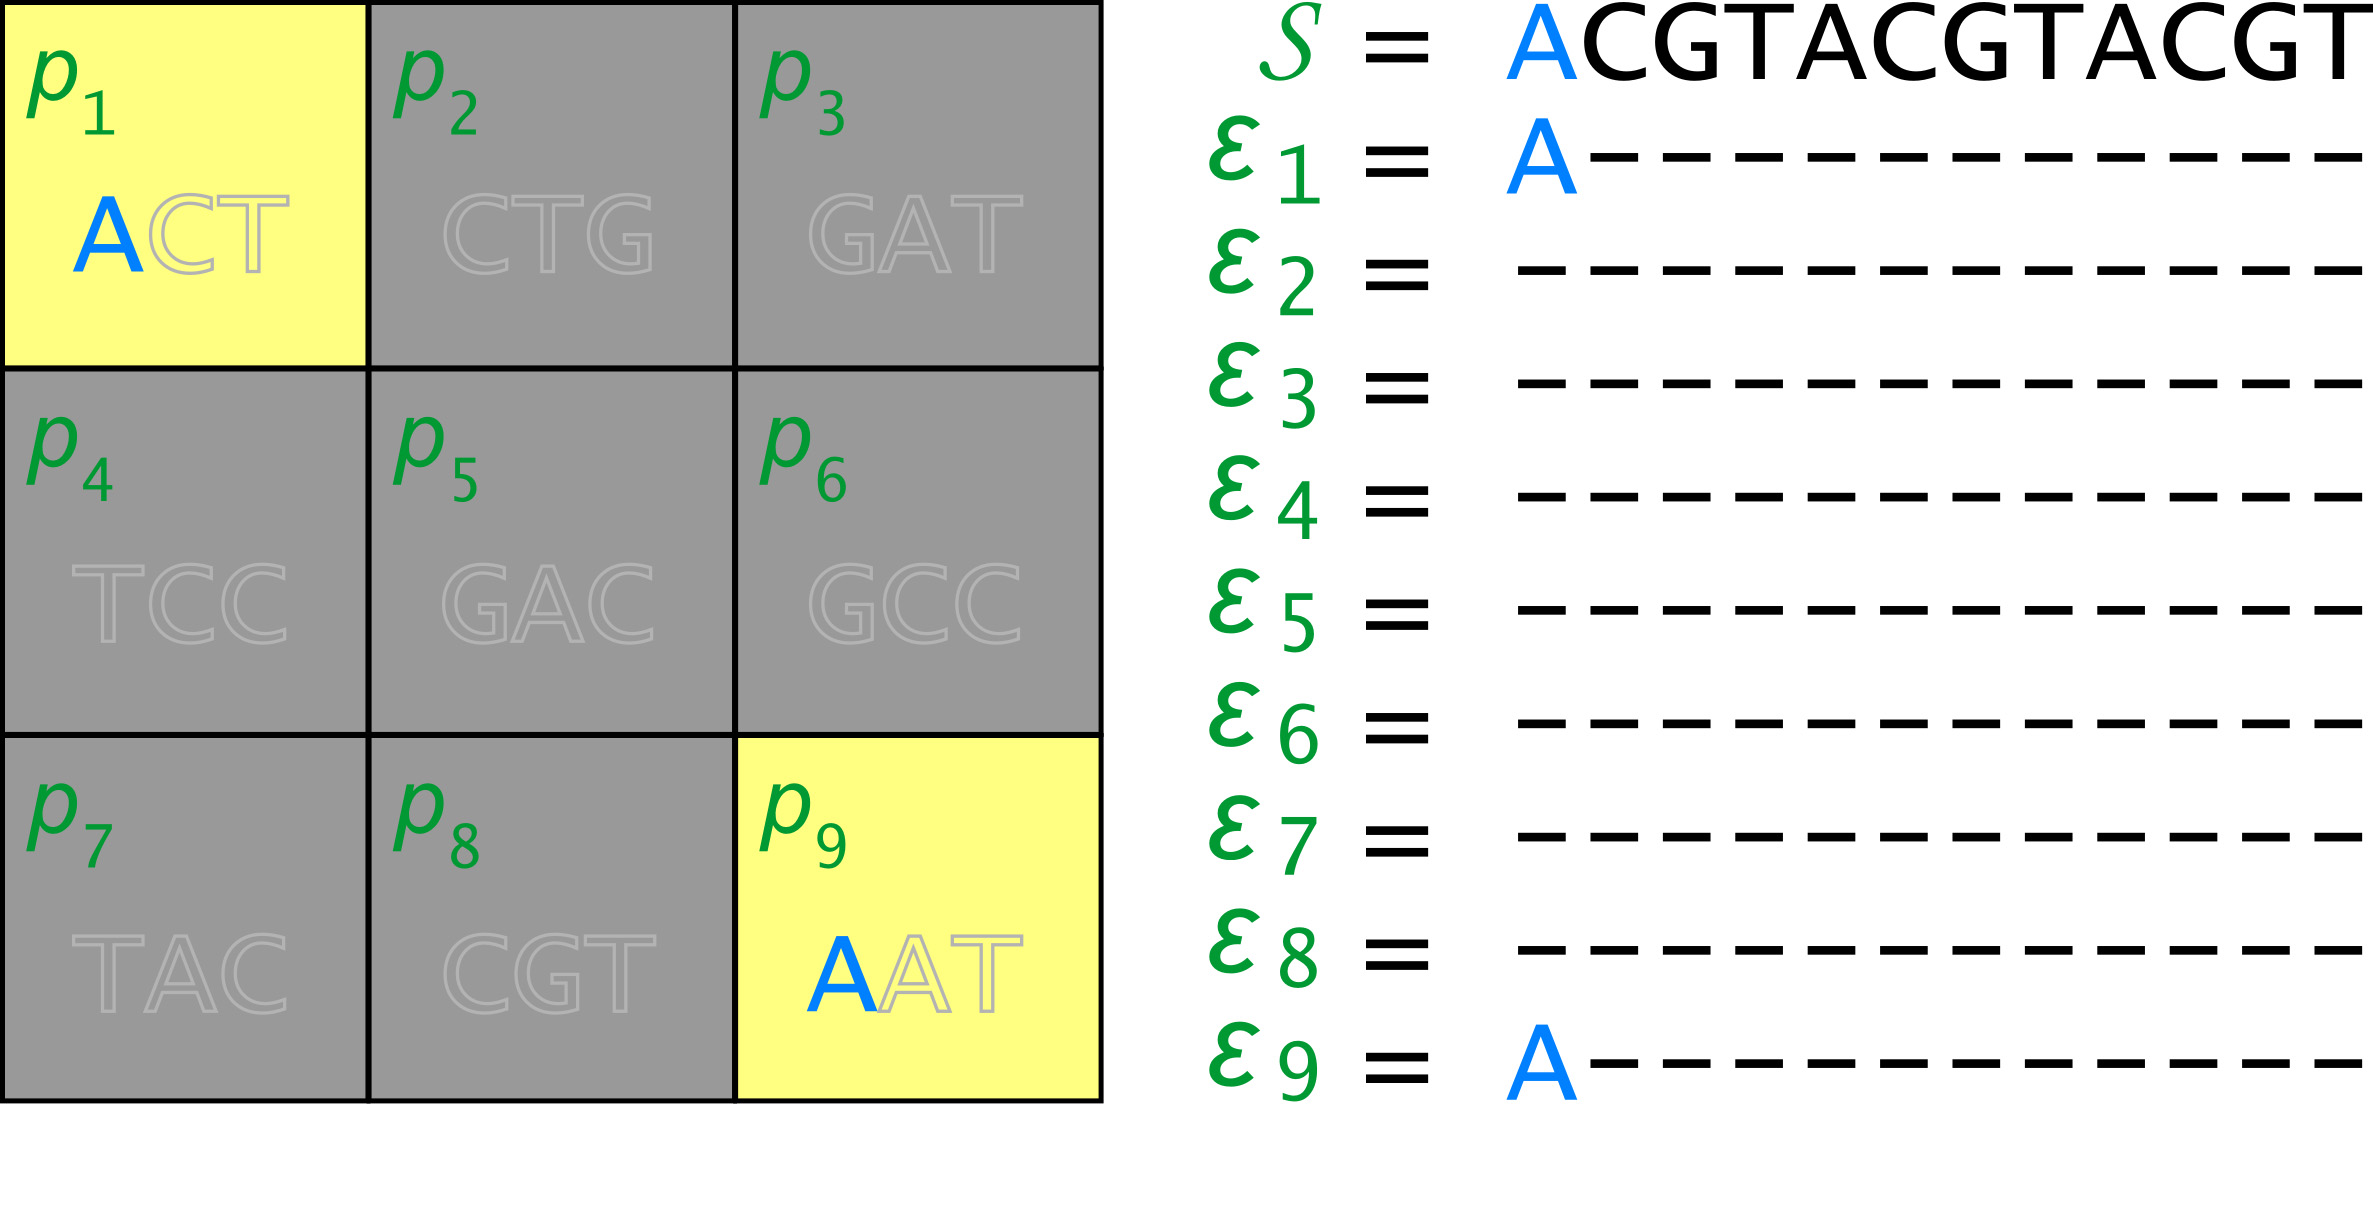
\includegraphics[width=\textwidth]{masks/mask1.jpg}
  \onslide<+>
    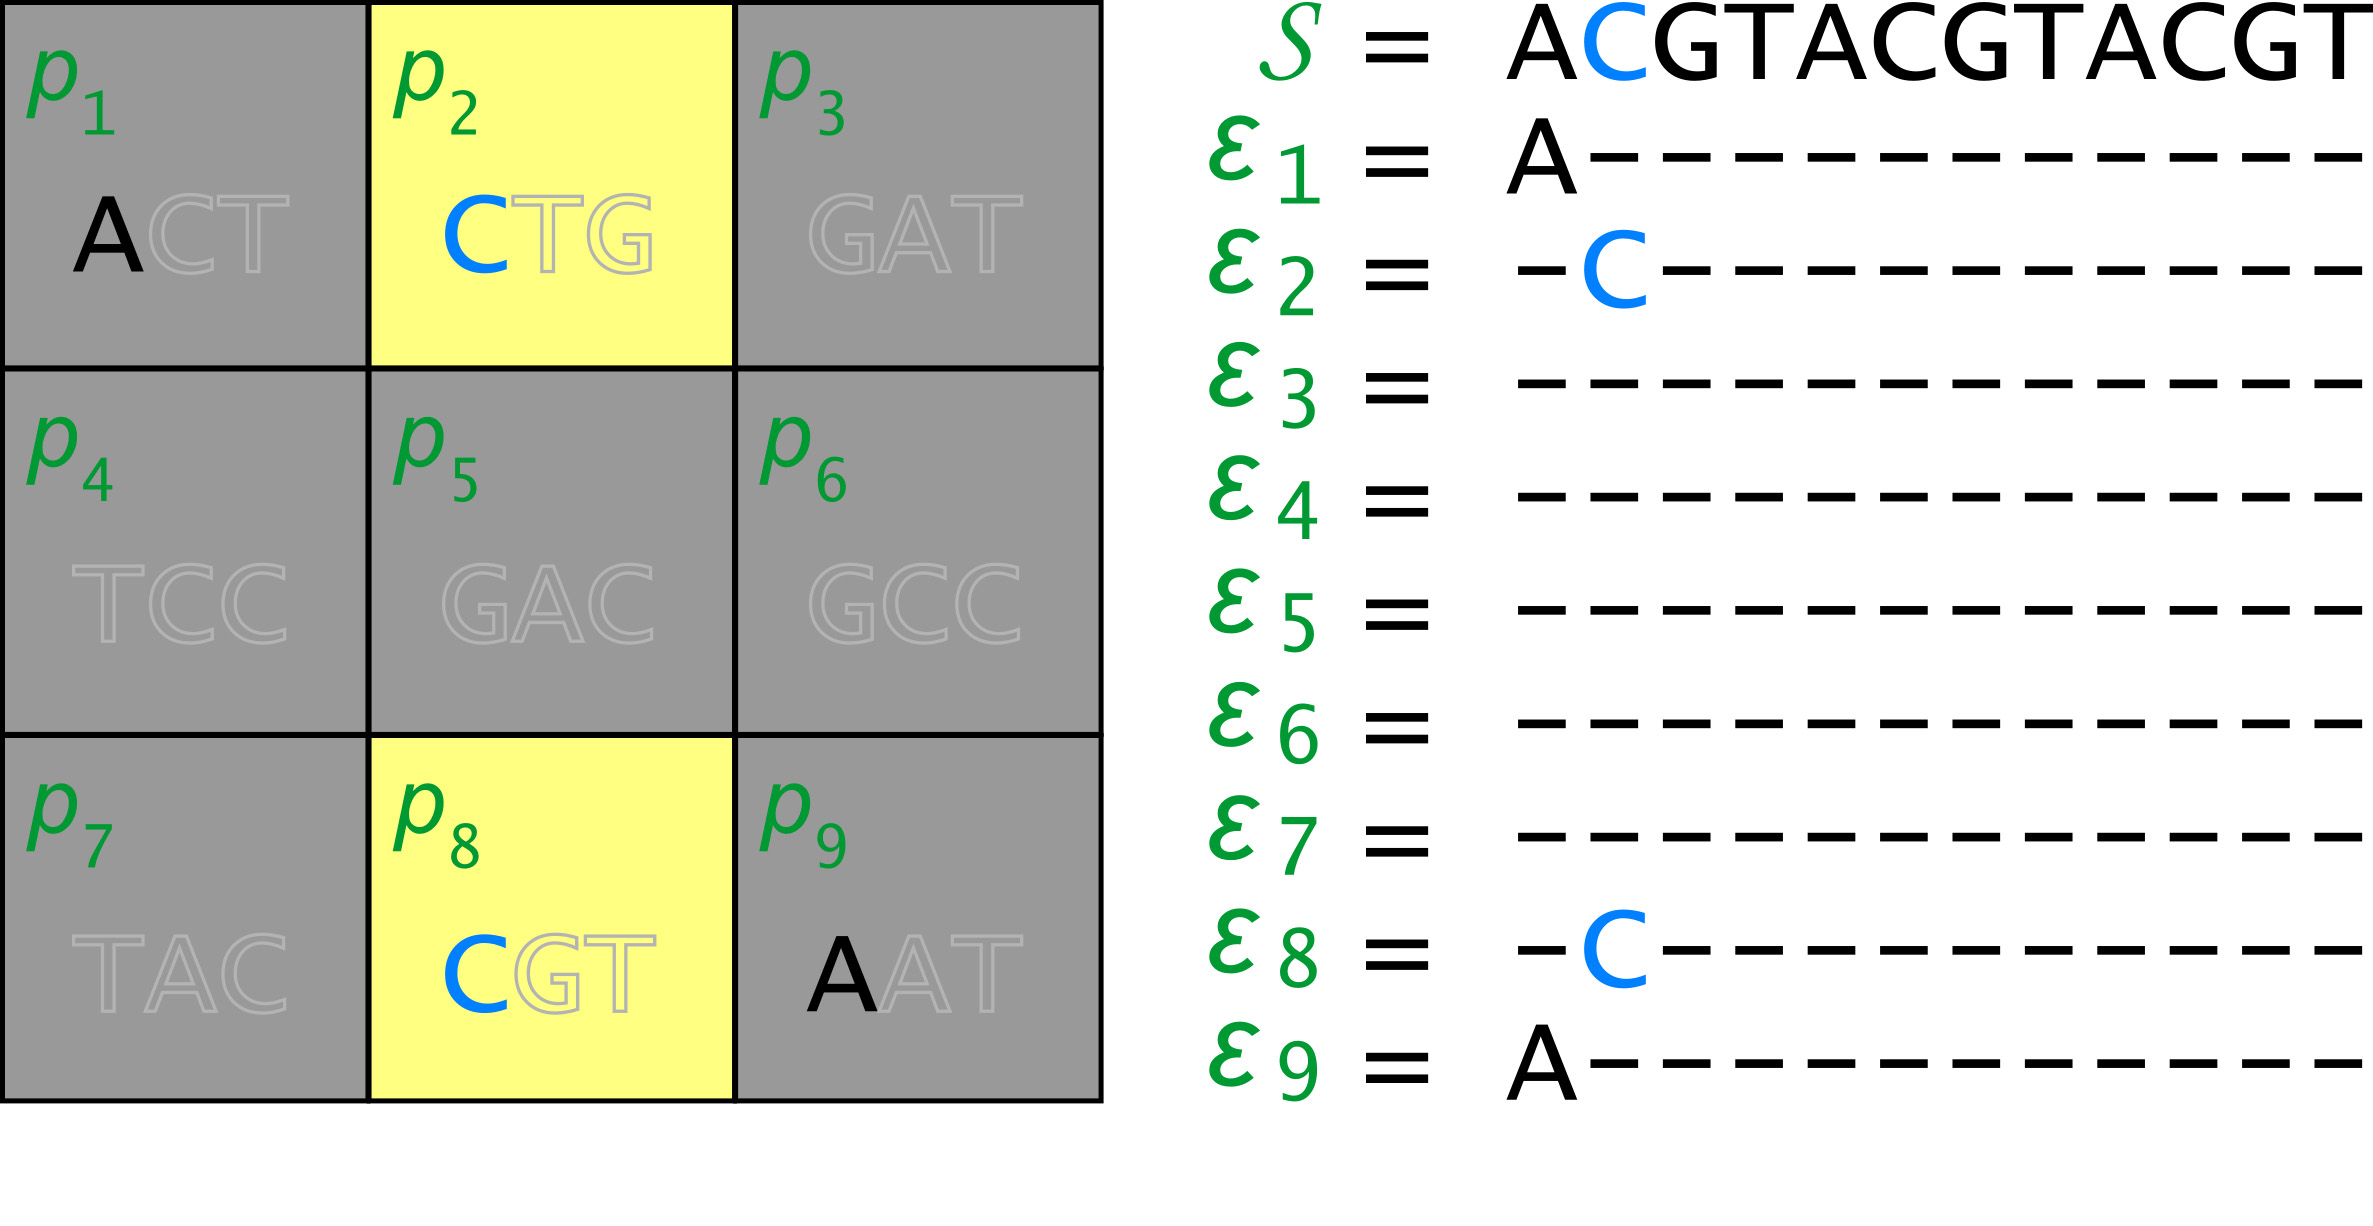
\includegraphics[width=\textwidth]{masks/mask2.jpg}
  \onslide<+>
    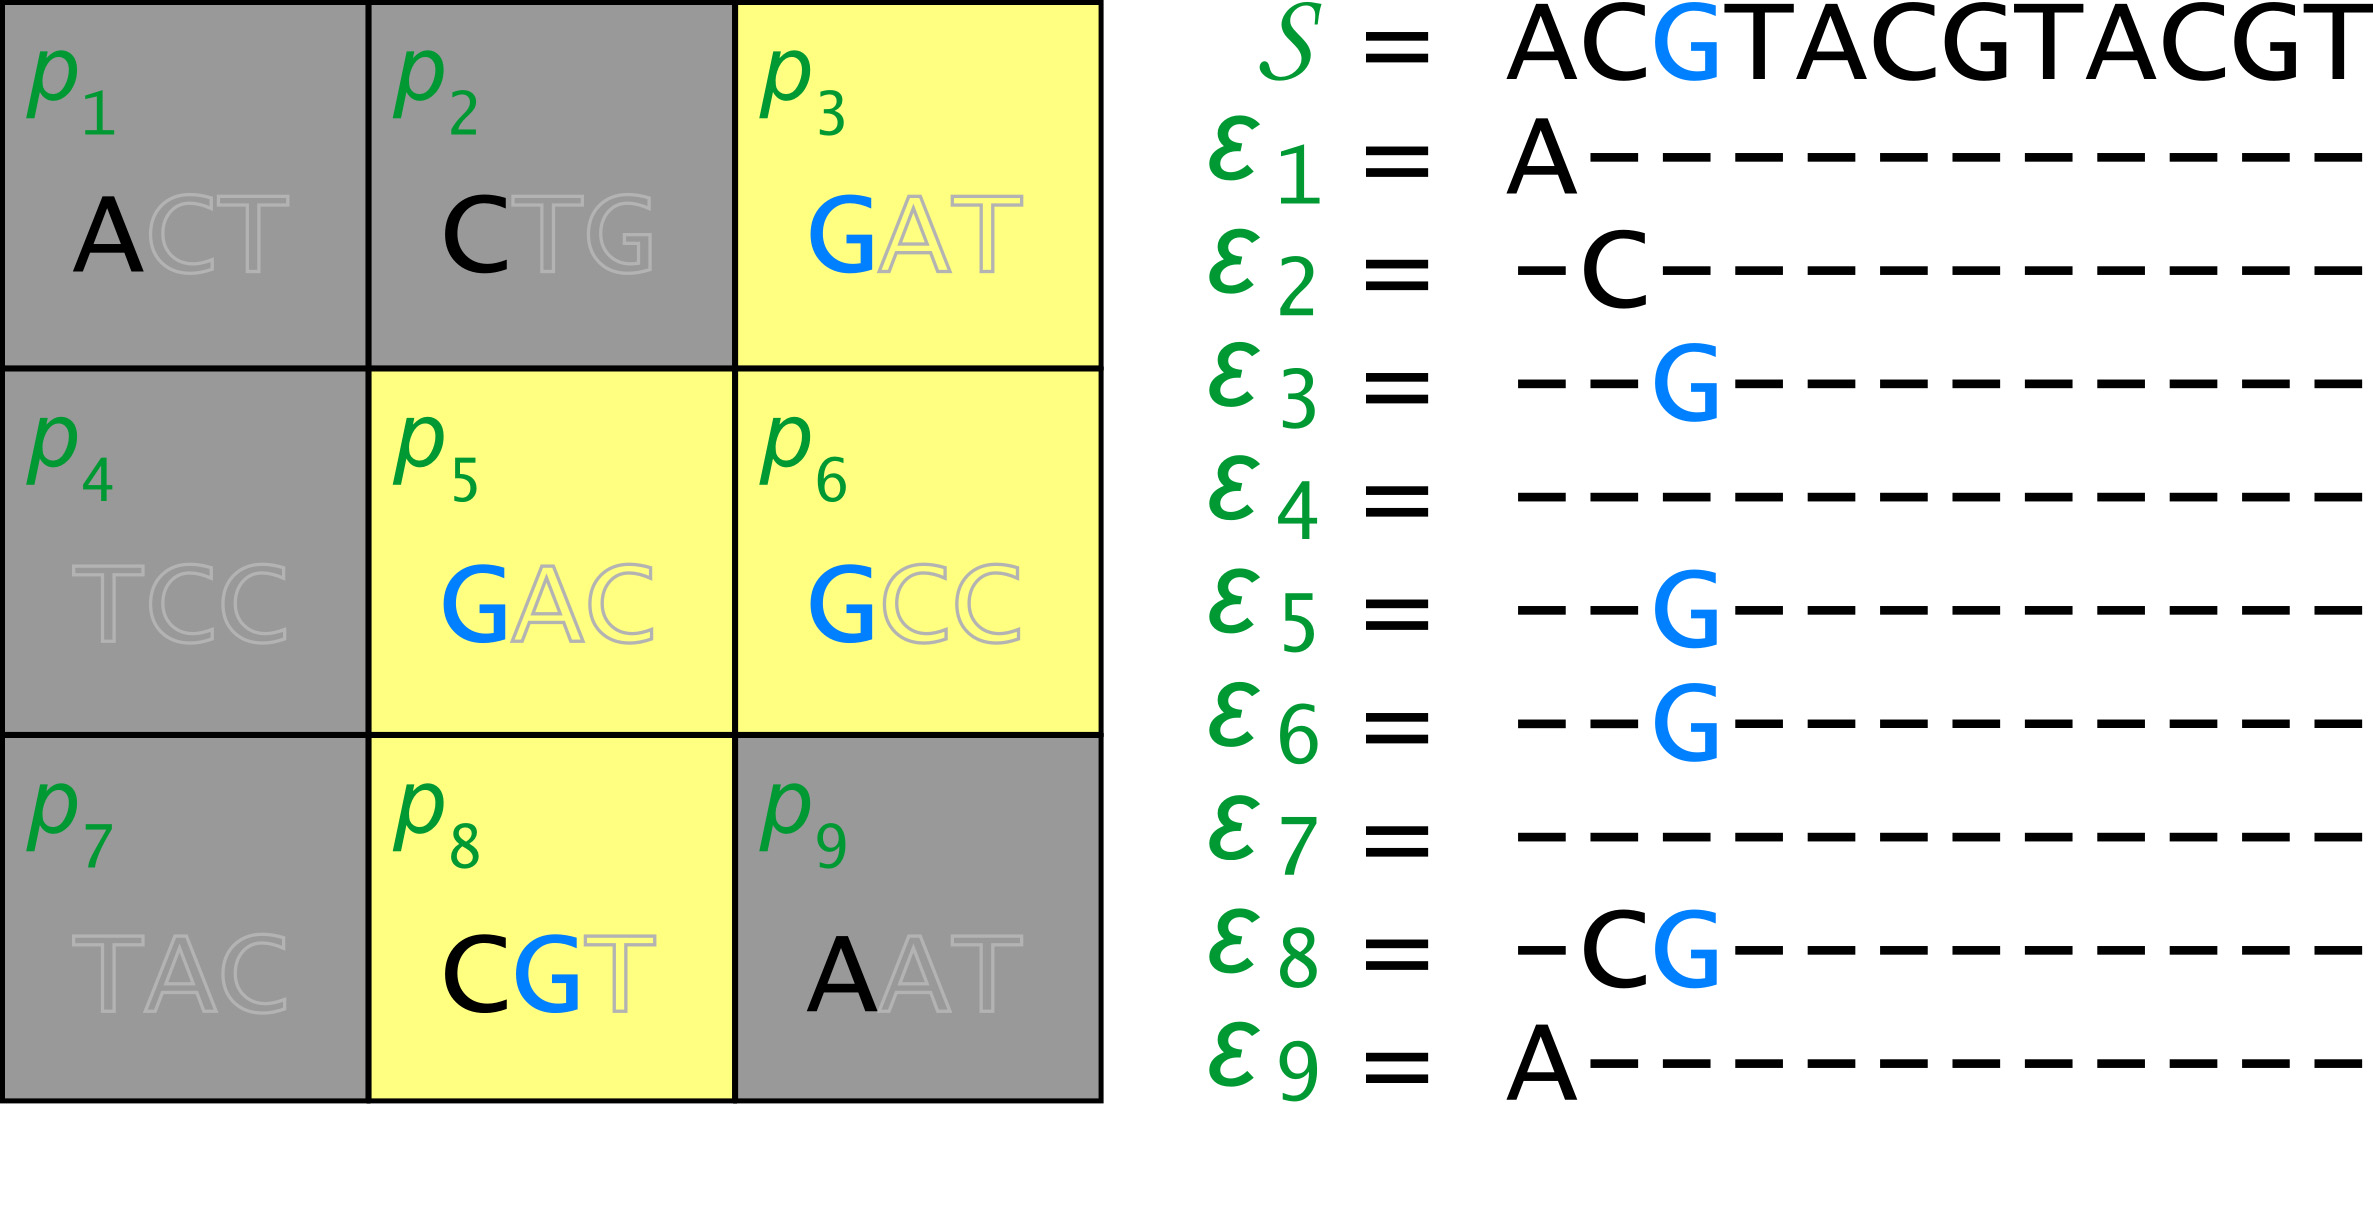
\includegraphics[width=\textwidth]{masks/mask3.jpg}
  \onslide<+>
    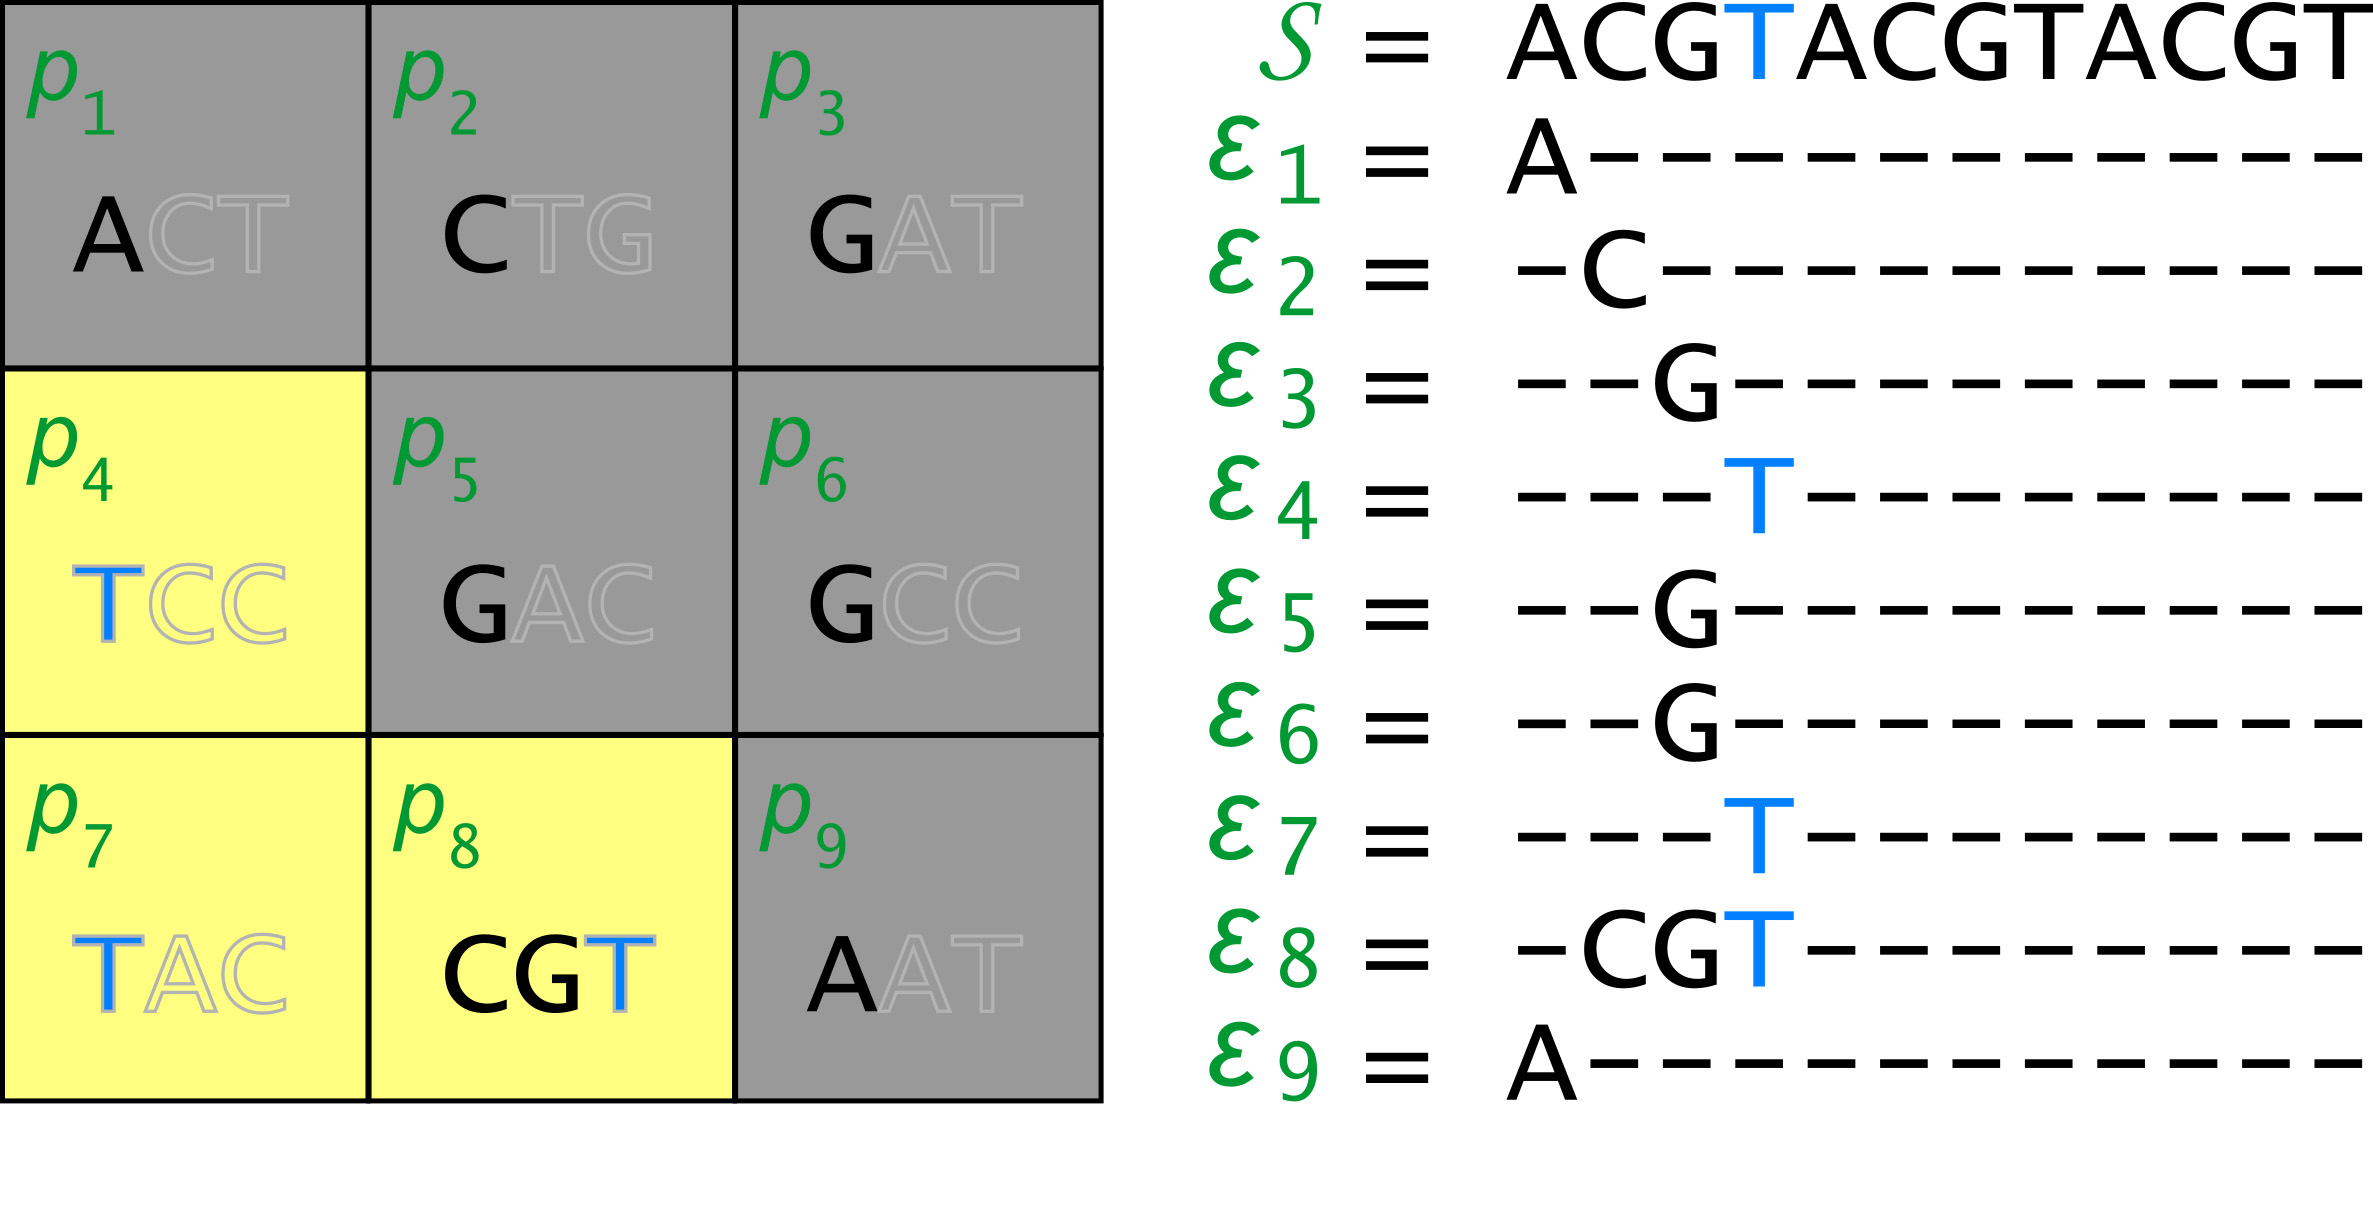
\includegraphics[width=\textwidth]{masks/mask4.jpg}
  \onslide<+>
    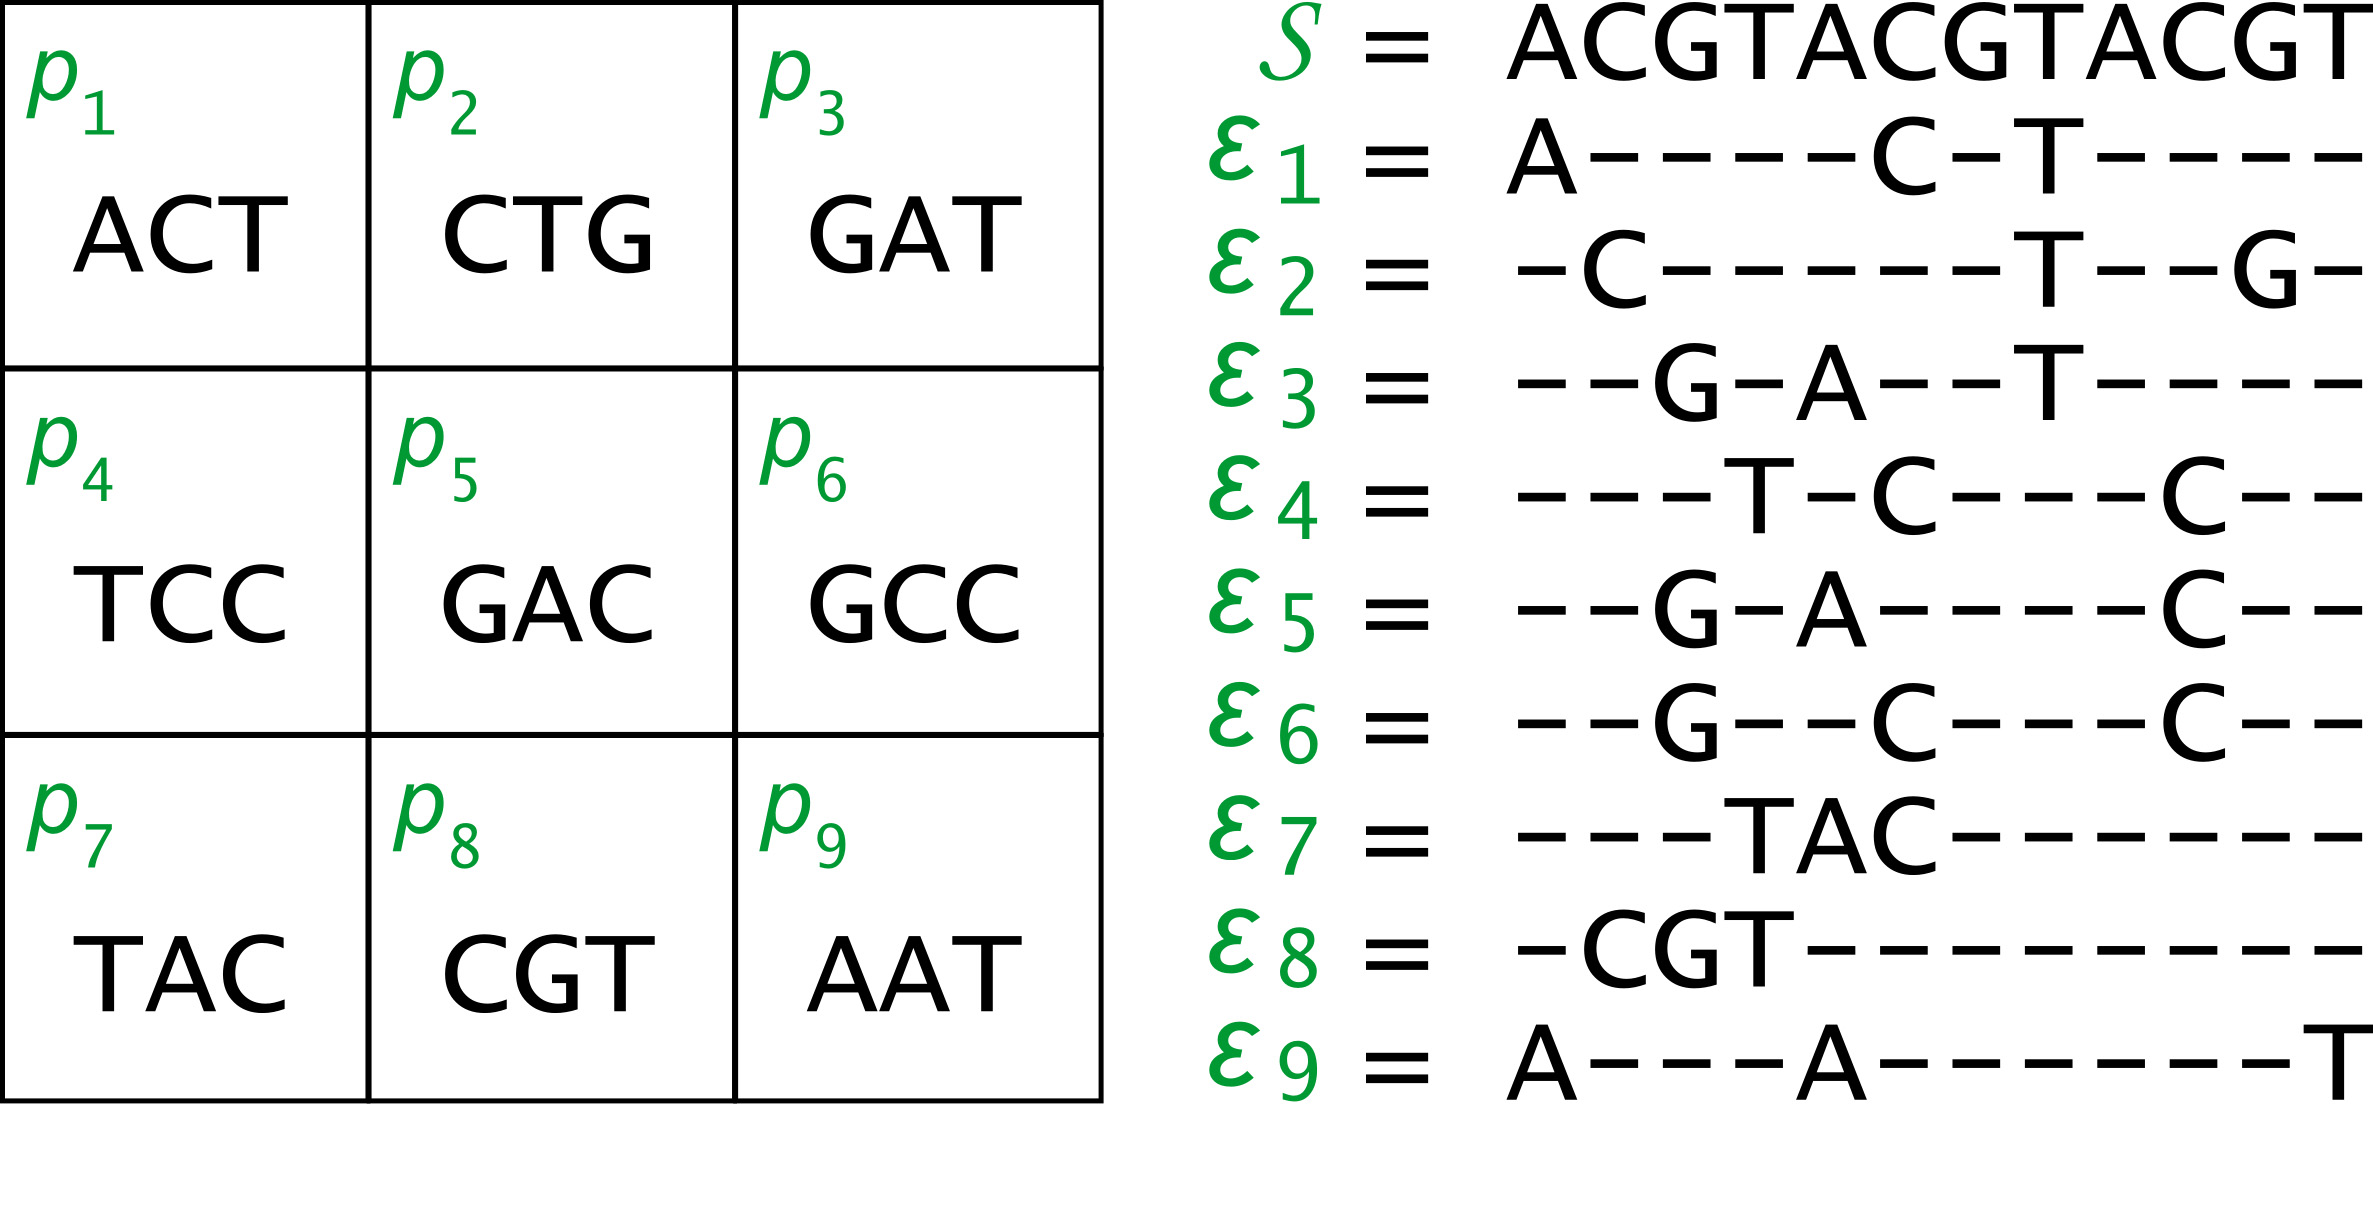
\includegraphics[width=\textwidth]{masks/embed.jpg}
  \onslide<+>
    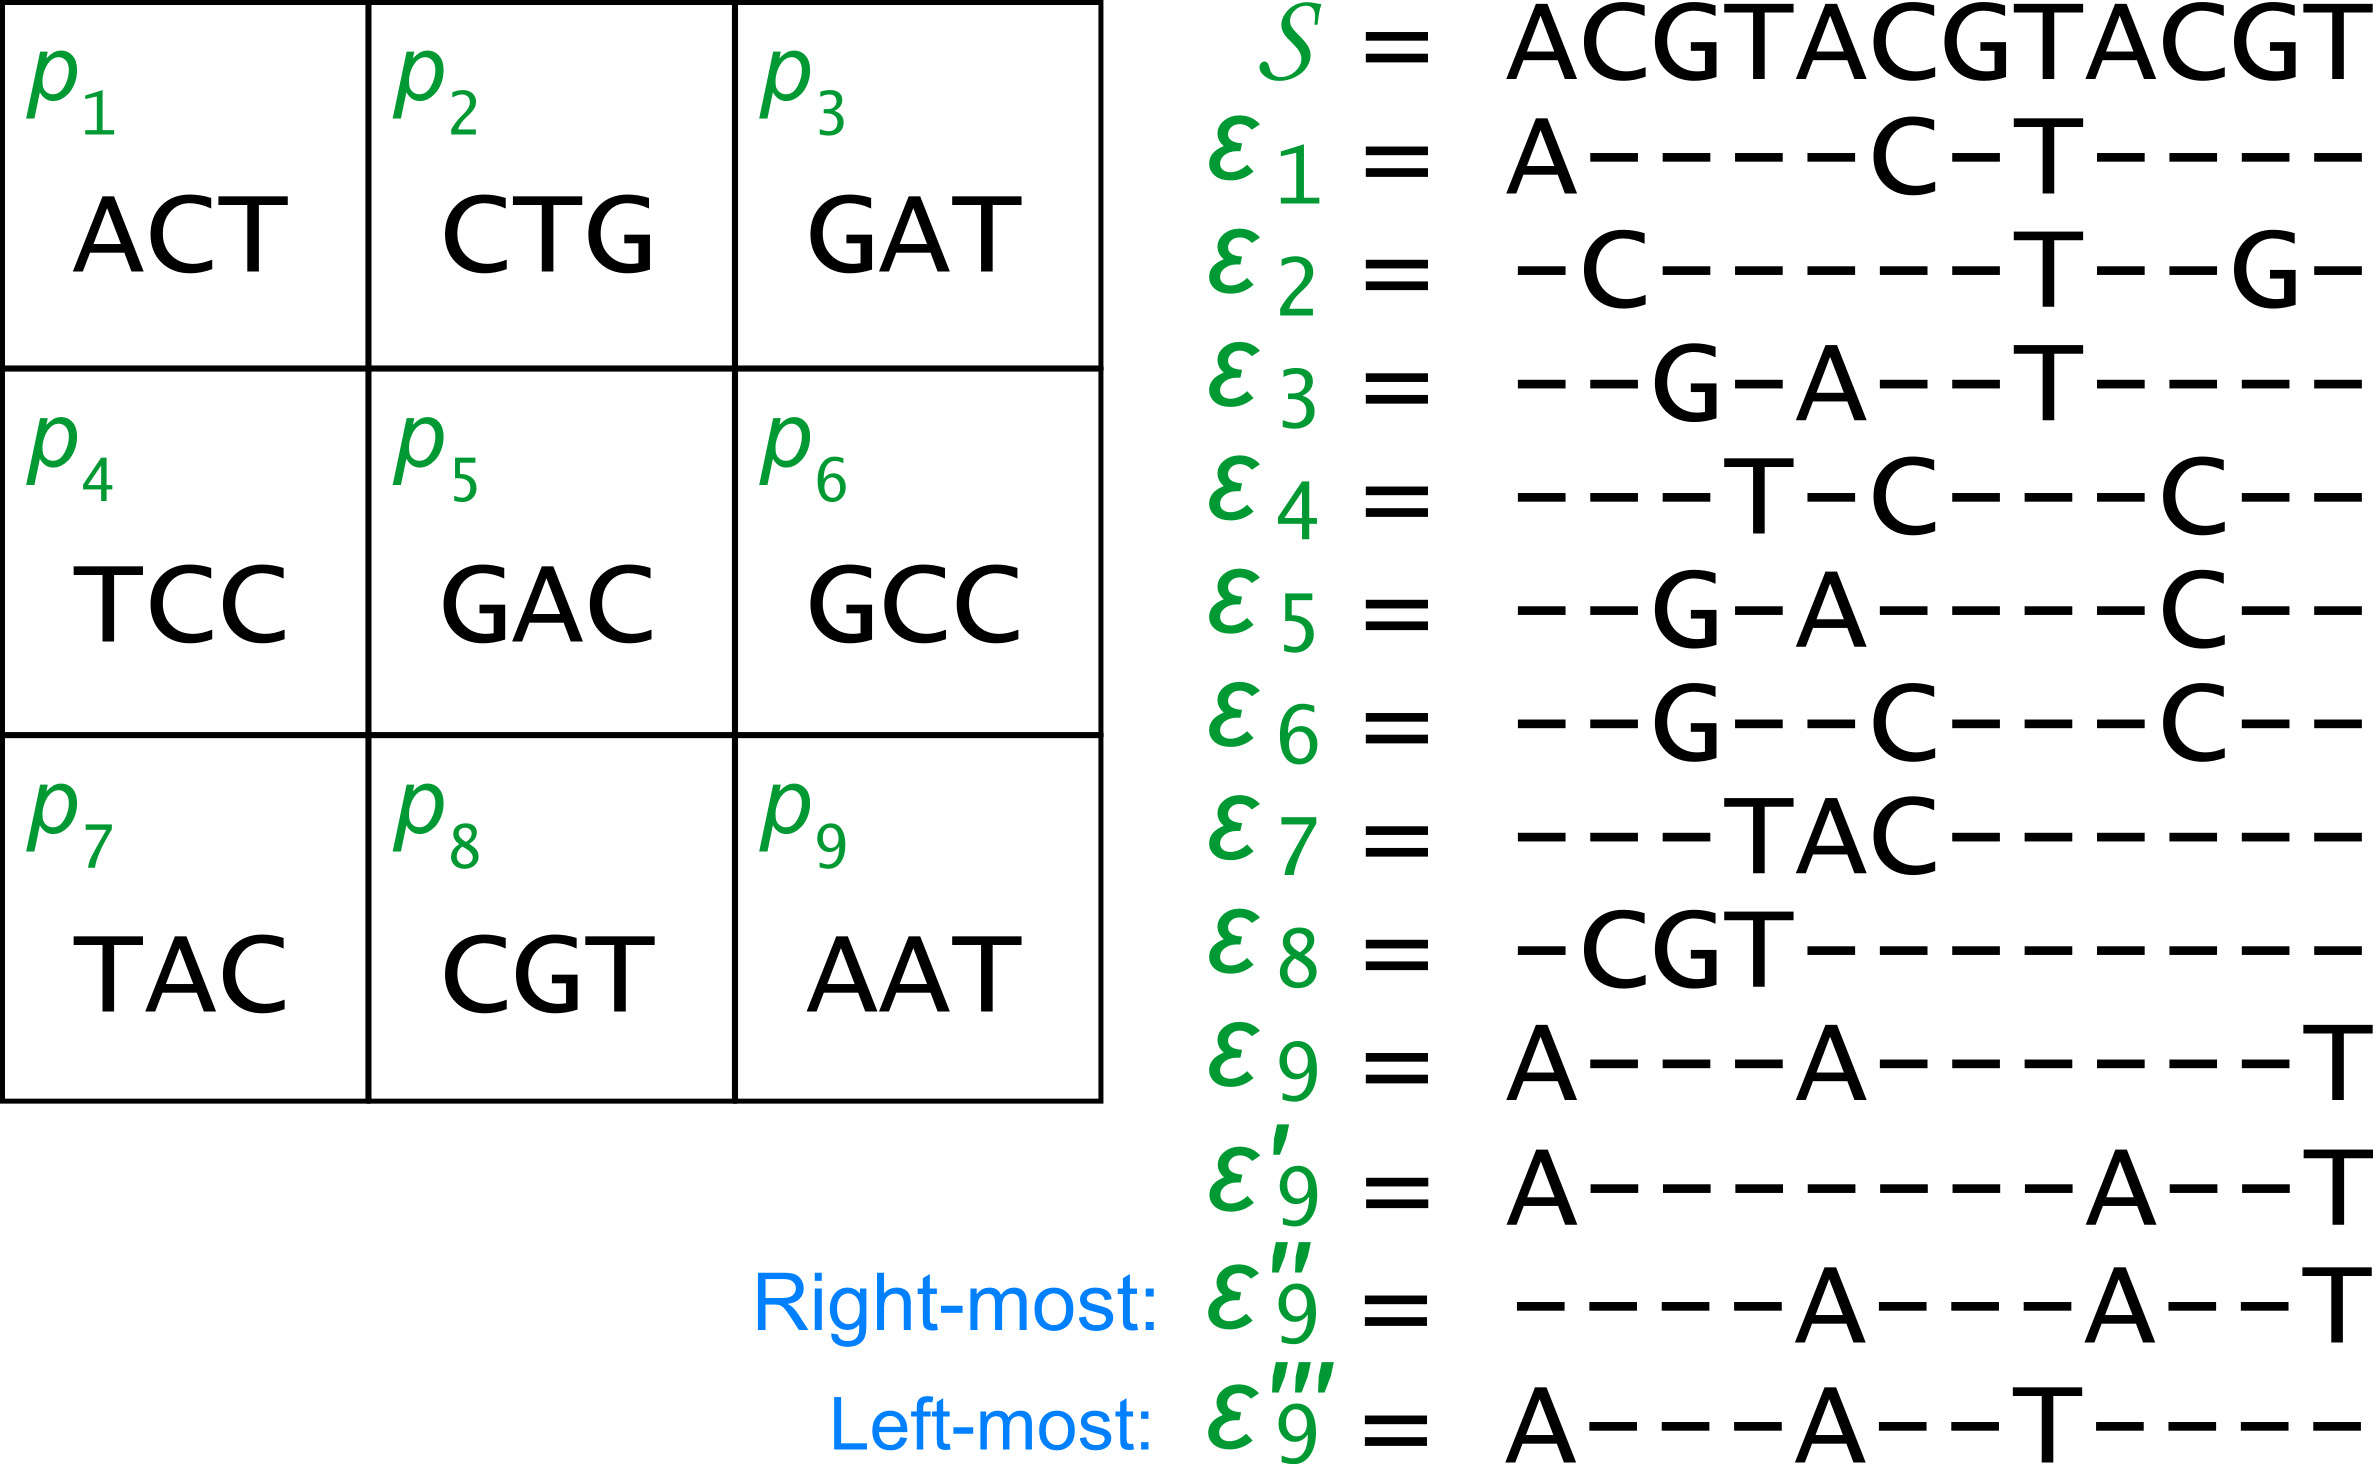
\includegraphics[width=\textwidth]{masks/alternatives.jpg}
  \end{overprint}

}

%%%%%%%%%%%%%%%%%%%%%%%%%%%%%%%%%%%%%%%%%%%%%%%%%%%%%%%%%%%%%%%%%%%%%%%%%%%%%%%%
\frame[label=problem]{\frametitle{Unintended Illumination Problem}

  \begin{columns}
  
    \begin{column}{0.45\textwidth}
      \centerline{
        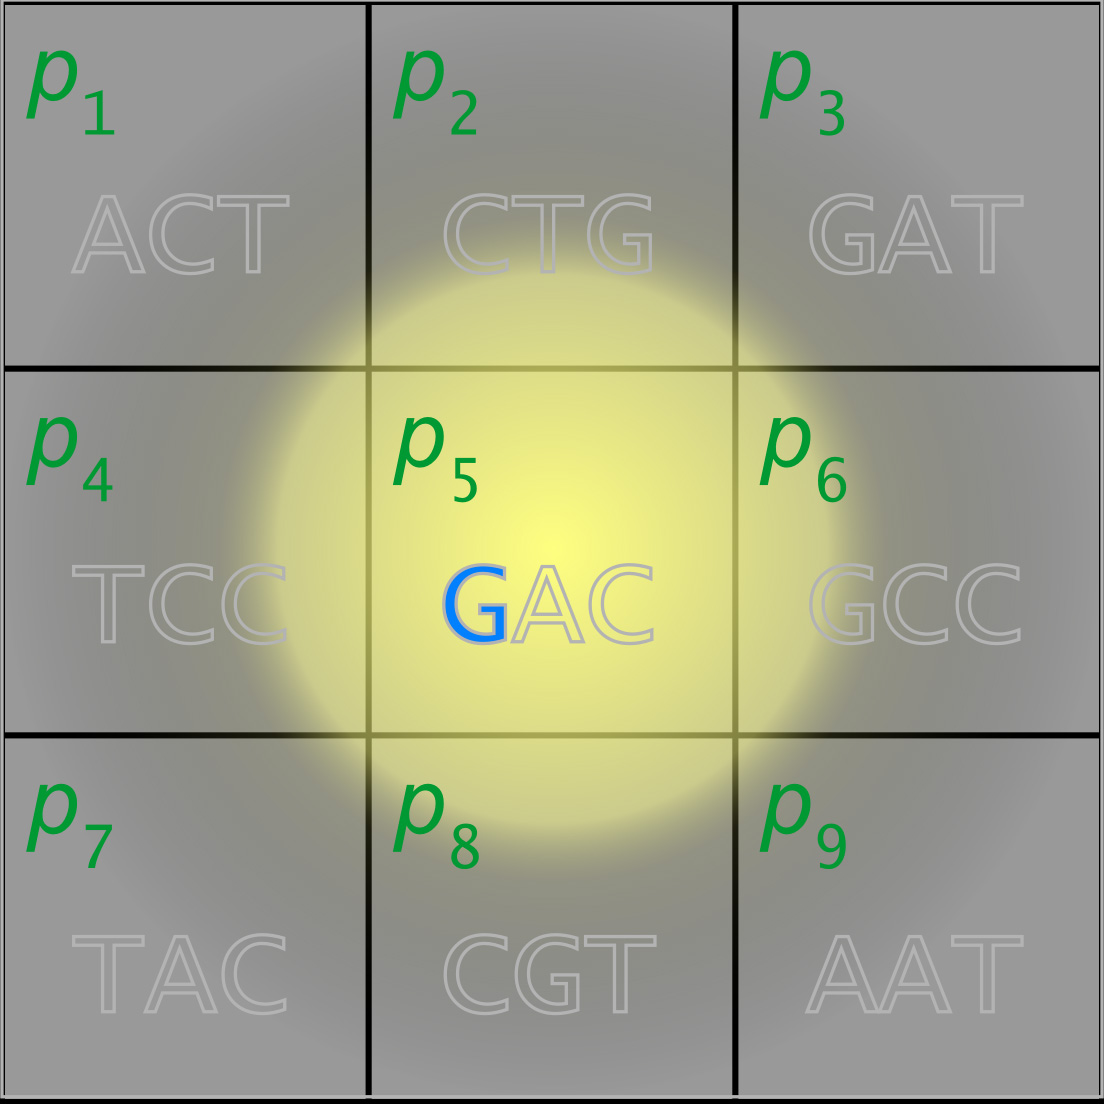
\includegraphics[width=\textwidth]{pics/straylight.jpg}
      }
    \end{column}
    
    \begin{column}{0.55\textwidth}
      \begin{itemize}
        \item \alert{Untargeted spots} can be accidentally activated
        \begin{itemize}
          \item Diffraction of light
          \item Internal reflection
        \end{itemize}
        \item Production of defective probes
        \item More likely near the \alert{borders} between masked and unmasked
              spots: \alert{border conflict}
      \end{itemize}
    \end{column}
    
  \end{columns}
  
  \begin{block}{Border Length Minimization Problem (Hannenhalli et al., 2002)}
    \begin{itemize}
      \item Find arrangement (and embeddings) with minimum number of border
            conflicts
    \end{itemize}
  \end{block}

}

%% *****************************************************************************
\section[Conflict Index]{Conflict Index Model}
\subsection{Dummy}
%% *****************************************************************************

%%%%%%%%%%%%%%%%%%%%%%%%%%%%%%%%%%%%%%%%%%%%%%%%%%%%%%%%%%%%%%%%%%%%%%%%%%%%%%%%
\frame{\frametitle{Motivation}

  \begin{columns}  
  
    \begin{column}{0.55\textwidth}
      \begin{itemize}
        \item Border Length measures the quality of a particular mask
        \begin{itemize}
          \item We are more interested in a \alert{per-probe measure}
        \end{itemize}
        \item Practical considerations need to be taken into account:
        \begin{itemize}
          \item[a)] Stray light might damage probes that lie as far as \alert{three
                    cells away} from the targeted spot
          \item[b)] Imperfections produced \alert{in the middle} of a probe are more
                    harmful than in its extremities
        \end{itemize}
      \end{itemize}
    \end{column}
      
    \begin{column}{0.45\textwidth}
      \centerline{
        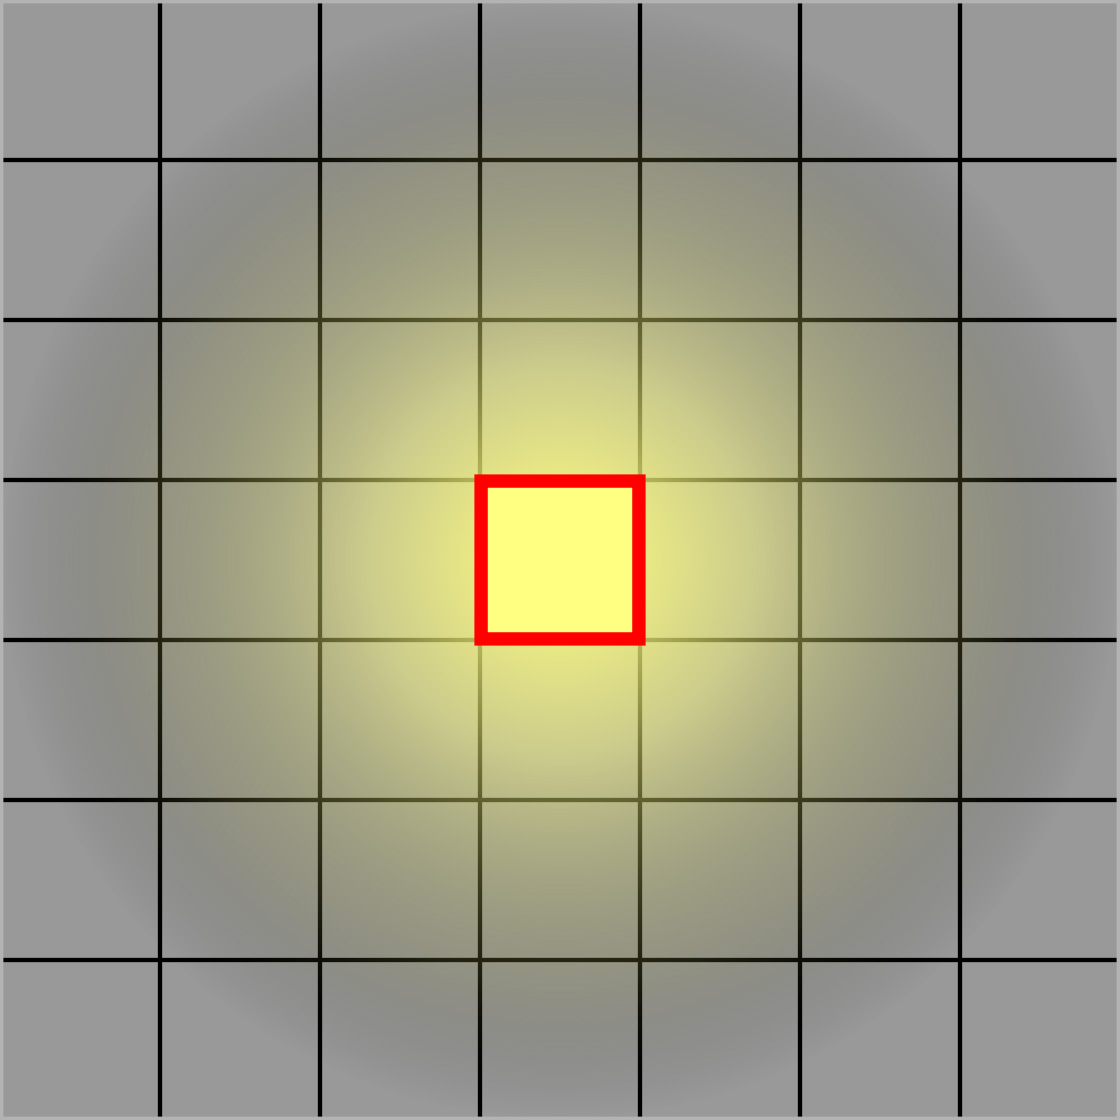
\includegraphics[width=\textwidth]{pics/distance.jpg}
      }
    \end{column}
  
  \end{columns}
  
  \vspace*{0.35cm}
  
\includegraphics[width=\textwidth]{pics/position.jpg}
}

%%%%%%%%%%%%%%%%%%%%%%%%%%%%%%%%%%%%%%%%%%%%%%%%%%%%%%%%%%%%%%%%%%%%%%%%%%%%%%%%
\frame{\frametitle{Definition}

  \begin{block}{Conflict Index of a probe $p$}
    \footnotesize{
    \[
    \mathcal{C}(p) := \sum_{t=1}^{T} \Bigl( \omega(p,t) \sum_{p'} \delta(p,p',t) \Bigr)
    \]
    }
  \end{block}
    
  \begin{block}{Distance-dependent weights}
    \footnotesize{
    \[
    \delta(p,p',t) :=
    \left\{
    \begin{array}{ll}
    (d(p,p'))^{-2} & \mbox{if $p'$ is unmasked at step $t$}, \\
                 0 & \mbox{otherwise}, \\
    \end{array}
    \right.
    \]
    %%
    where $d(p,p')$ is the \alert{Euclidean distance} between the spots of~$p$
    and~$p'$.
    }
  \end{block}

  \vspace*{0.2cm}

  \centerline{
  \scriptsize{
  \begin{tabular}{|c|c|c|c|c|c|c|c|} \hline
  0.06 & 0.08 & 0.10 & 0.11 & 0.10 & 0.08 & 0.06 \\ \hline
  0.08 & 0.13 & 0.20 & 0.25 & 0.20 & 0.13 & 0.08 \\ \hline
  0.10 & 0.20 & 0.50 & 1.00 & 0.50 & 0.20 & 0.10 \\ \hline
  0.11 & 0.25 & 1.00 & \alert{$p$} & 1.00 & 0.25 & 0.11 \\ \hline
  0.10 & 0.20 & 0.50 & 1.00 & 0.50 & 0.20 & 0.10 \\ \hline
  0.08 & 0.13 & 0.20 & 0.25 & 0.20 & 0.13 & 0.08 \\ \hline
  0.06 & 0.08 & 0.10 & 0.11 & 0.10 & 0.08 & 0.06 \\ \hline
  \end{tabular}}}
  
}

%%%%%%%%%%%%%%%%%%%%%%%%%%%%%%%%%%%%%%%%%%%%%%%%%%%%%%%%%%%%%%%%%%%%%%%%%%%%%%%%
\frame{\frametitle{Definition}

  \begin{columns}
  
    \begin{column}{0.45\textwidth}
      \begin{block}{Conflict Index of a probe $p$}
        \footnotesize{
        \[
        \mathcal{C}(p) := \sum_{t=1}^{T} \Bigl( \omega(p,t) \sum_{p'} \delta(p,p',t) \Bigr)
        \]
        }
      \end{block}
    \end{column}
    
    \begin{column}{0.45\textwidth}
      \centerline{
        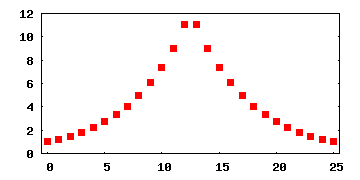
\includegraphics[width=1.25\textwidth]{pics/position_weights.png}
      }
    \end{column}
    
  \end{columns}

  \begin{block}{Position-dependent weights}
    \footnotesize{
    \[
    \omega(p,t) :=
    \left\{
    \begin{array}{ll}
    c \cdot \exp{\left(\theta \cdot \lambda(p,t)\right)} & \mbox{if $p$ is masked at step $t$}, \\
    0 & \mbox{otherwise}, \\
    \end{array}
    \right.
    \]
    %%
    where
    %%
    \[
    \lambda(p,t) := 1 + \min(b_{p,t},\ell_{p} - b_{p,t}),
    \]
    %%
    $b_{p,t}$ denotes the number of nucleotides synthesized up to and including
    step~$t$, $\ell_{p}$ is the length of probe~$p$, $c>0$ and $\theta>0$ are
    constants.
    }
  \end{block}

}

%% *****************************************************************************
\section[Pivot Partitioning]{Pivot Partitioning Algorithm}
\subsection{Dummy}
%% *****************************************************************************

%%%%%%%%%%%%%%%%%%%%%%%%%%%%%%%%%%%%%%%%%%%%%%%%%%%%%%%%%%%%%%%%%%%%%%%%%%%%%%%%
\frame{\frametitle{Previous Work: Place and Re-embed}

  \begin{itemize}
    \item The microarray layout problem has been traditionally approached in two
          phases:
    \begin{itemize}
      \item[1)] \alert{Placement} of probes given a fixed embedding
      \item[2)] \alert{Re-embedding} of probes once a placement is fixed
    \end{itemize}
  \end{itemize}
  
  \begin{block}{Placement: Row-epitaxial (Kahng {\it et~al}., 2003)}
    \begin{itemize}
      \item Spots are filled in a pre-defined order
      \begin{itemize}
        \item Select probe from a list $Q$ such that conflicts with filled spots
              are minimized
      \end{itemize}
      \item Restrict the maximum size of $Q$ (e.g. $Q = 20\,000$)
    \end{itemize}
  \end{block}

  \begin{block}{Re-embedding: several algorithms (Kahng {\it et~al}., 2002, 2003)}
    \begin{itemize}
      \item All based on the Optimum Single Probe Embedding (OSPE)
      \begin{itemize}
        \item Re-embed a probe \alert{optimally} in regards to its neighbors
      \end{itemize}
      \item Difference is the order in which probes are re-embedded
    \end{itemize}
  \end{block}
  
}

%%%%%%%%%%%%%%%%%%%%%%%%%%%%%%%%%%%%%%%%%%%%%%%%%%%%%%%%%%%%%%%%%%%%%%%%%%%%%%%%
\frame{\frametitle{Optimum Single Probe Embedding (OSPE)}

  \begin{itemize}
    \item Designed for border length minimization (Kahng {\it et~al}.,2002)
    \begin{itemize}
      \item We extended it for conflict index minimization
    \end{itemize}
  \end{itemize}

  \begin{overprint}
    
    \onslide<+>
      \centerline{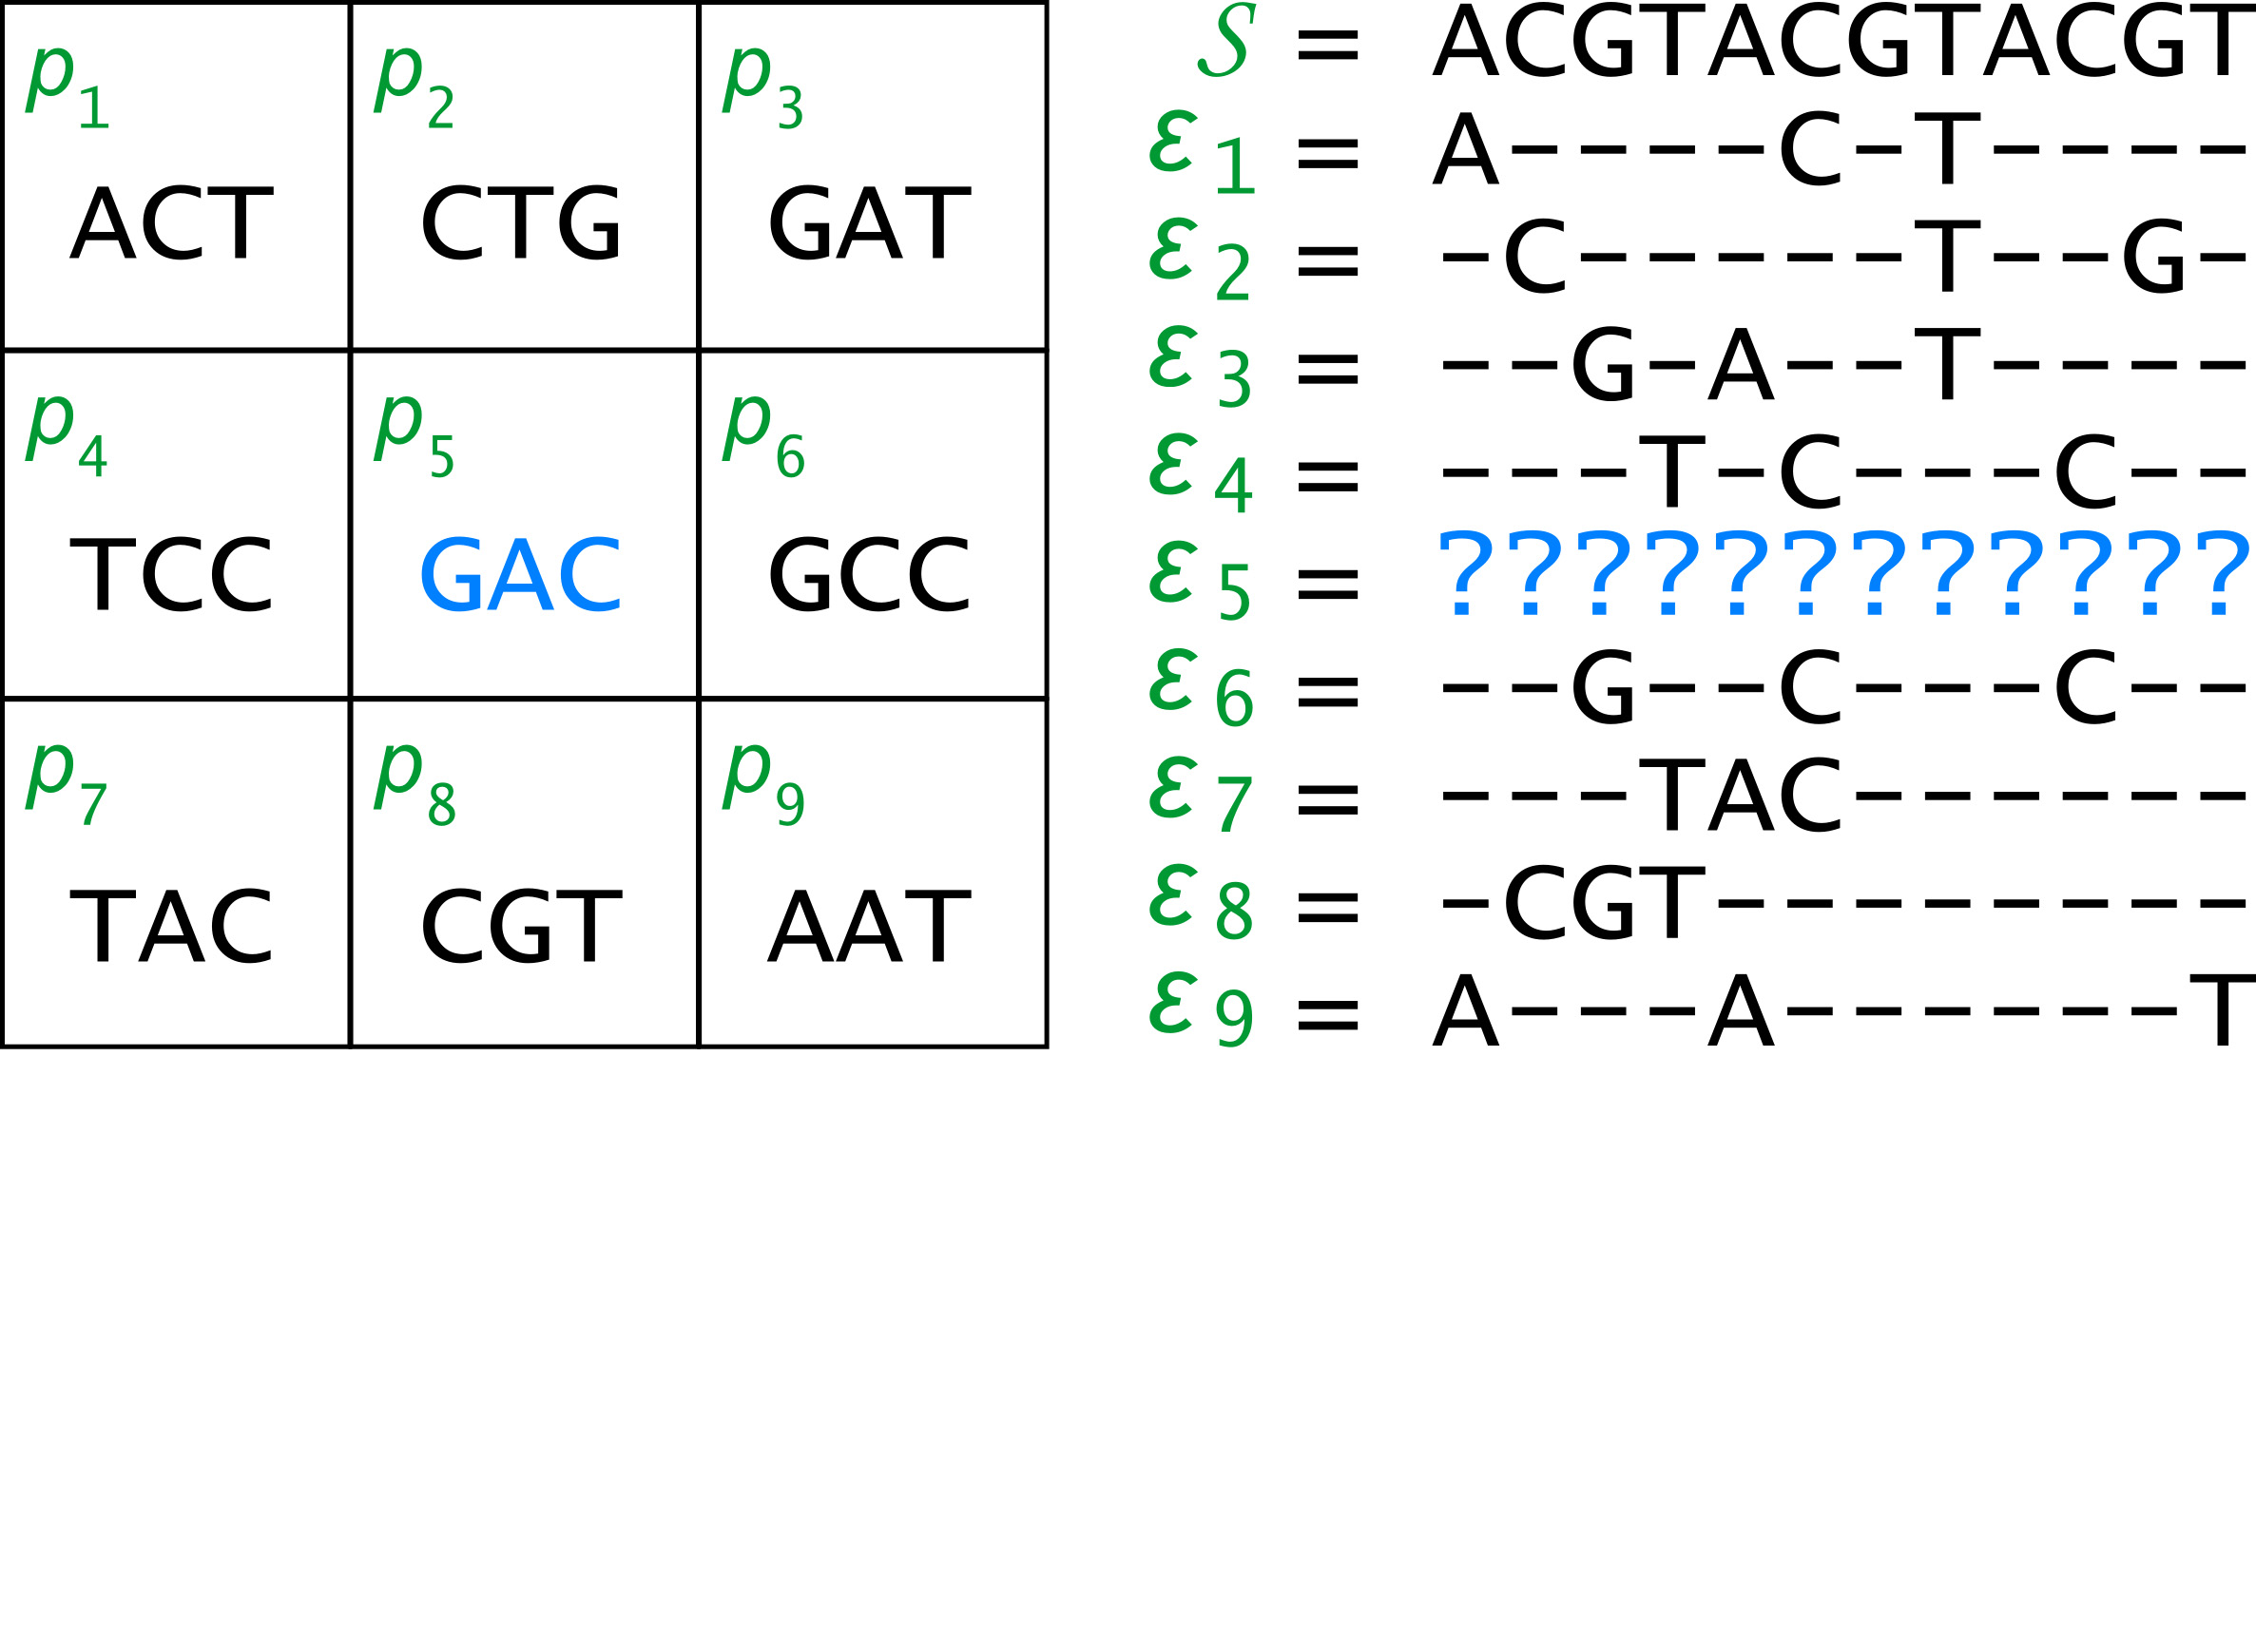
\includegraphics[width=0.8\textwidth]{pics/ospe0.jpg}}
    \onslide<+>
      \centerline{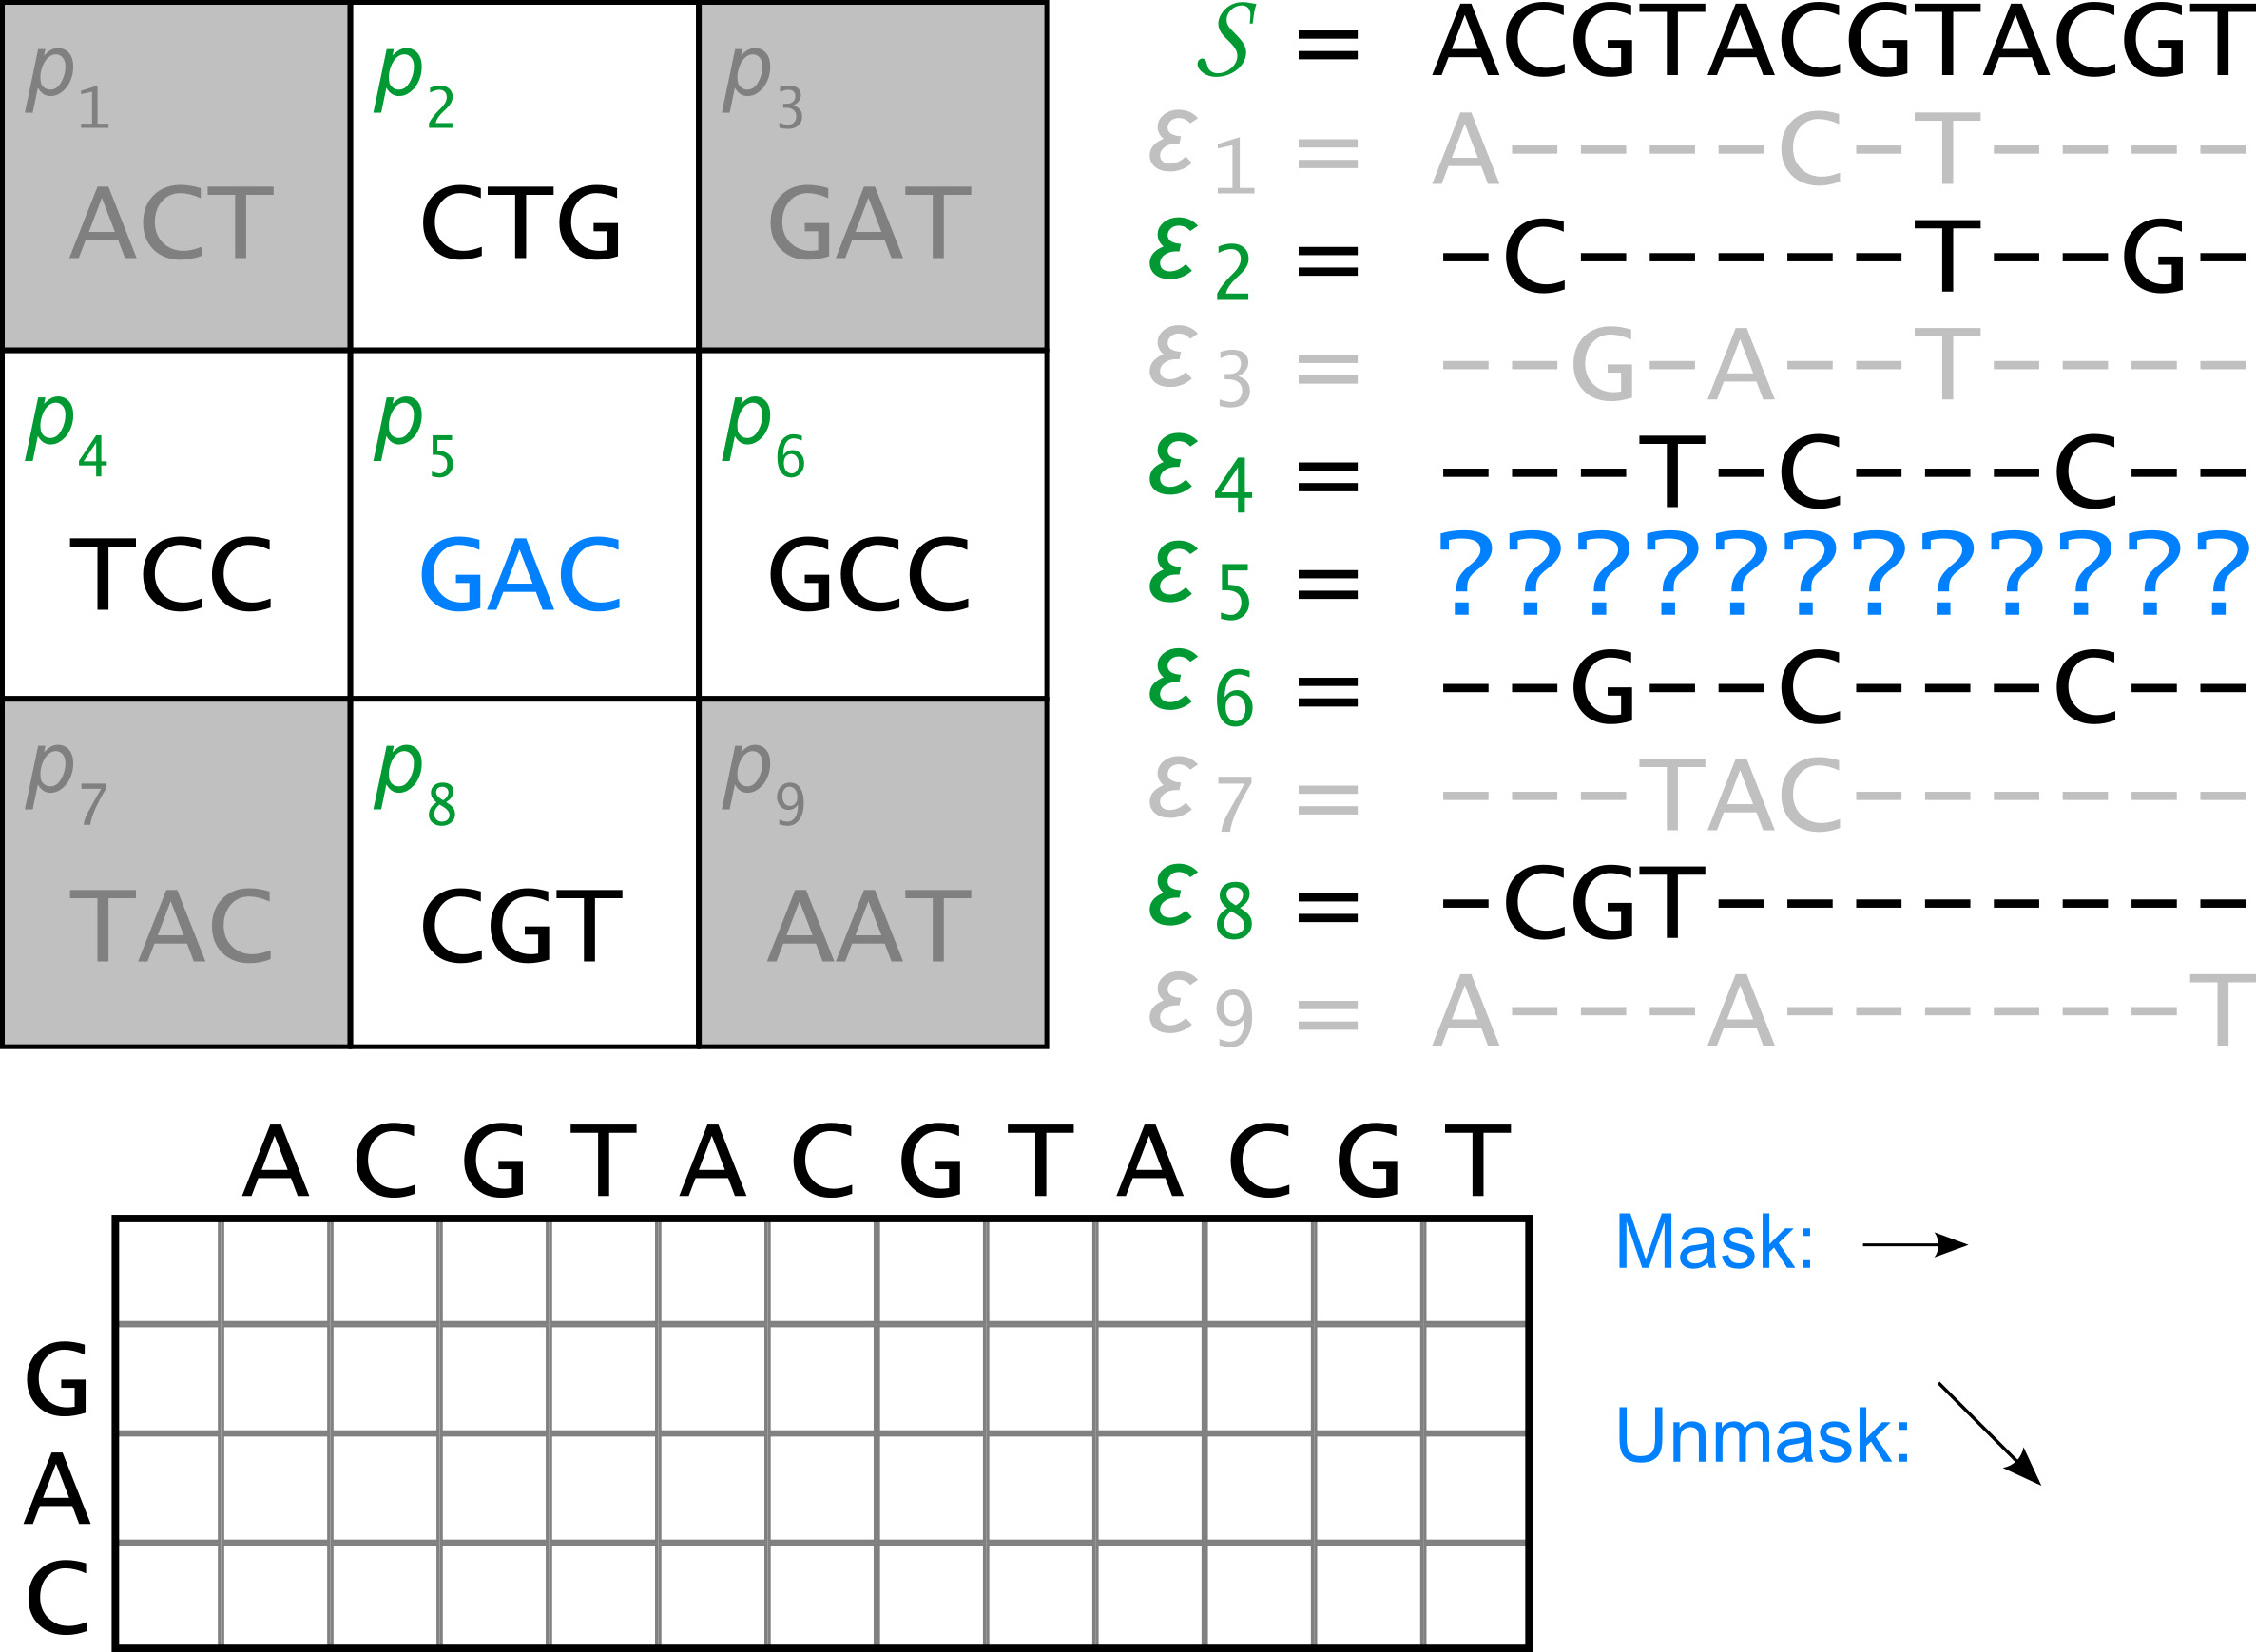
\includegraphics[width=0.8\textwidth]{pics/ospe1.jpg}}
    \onslide<+>
      \centerline{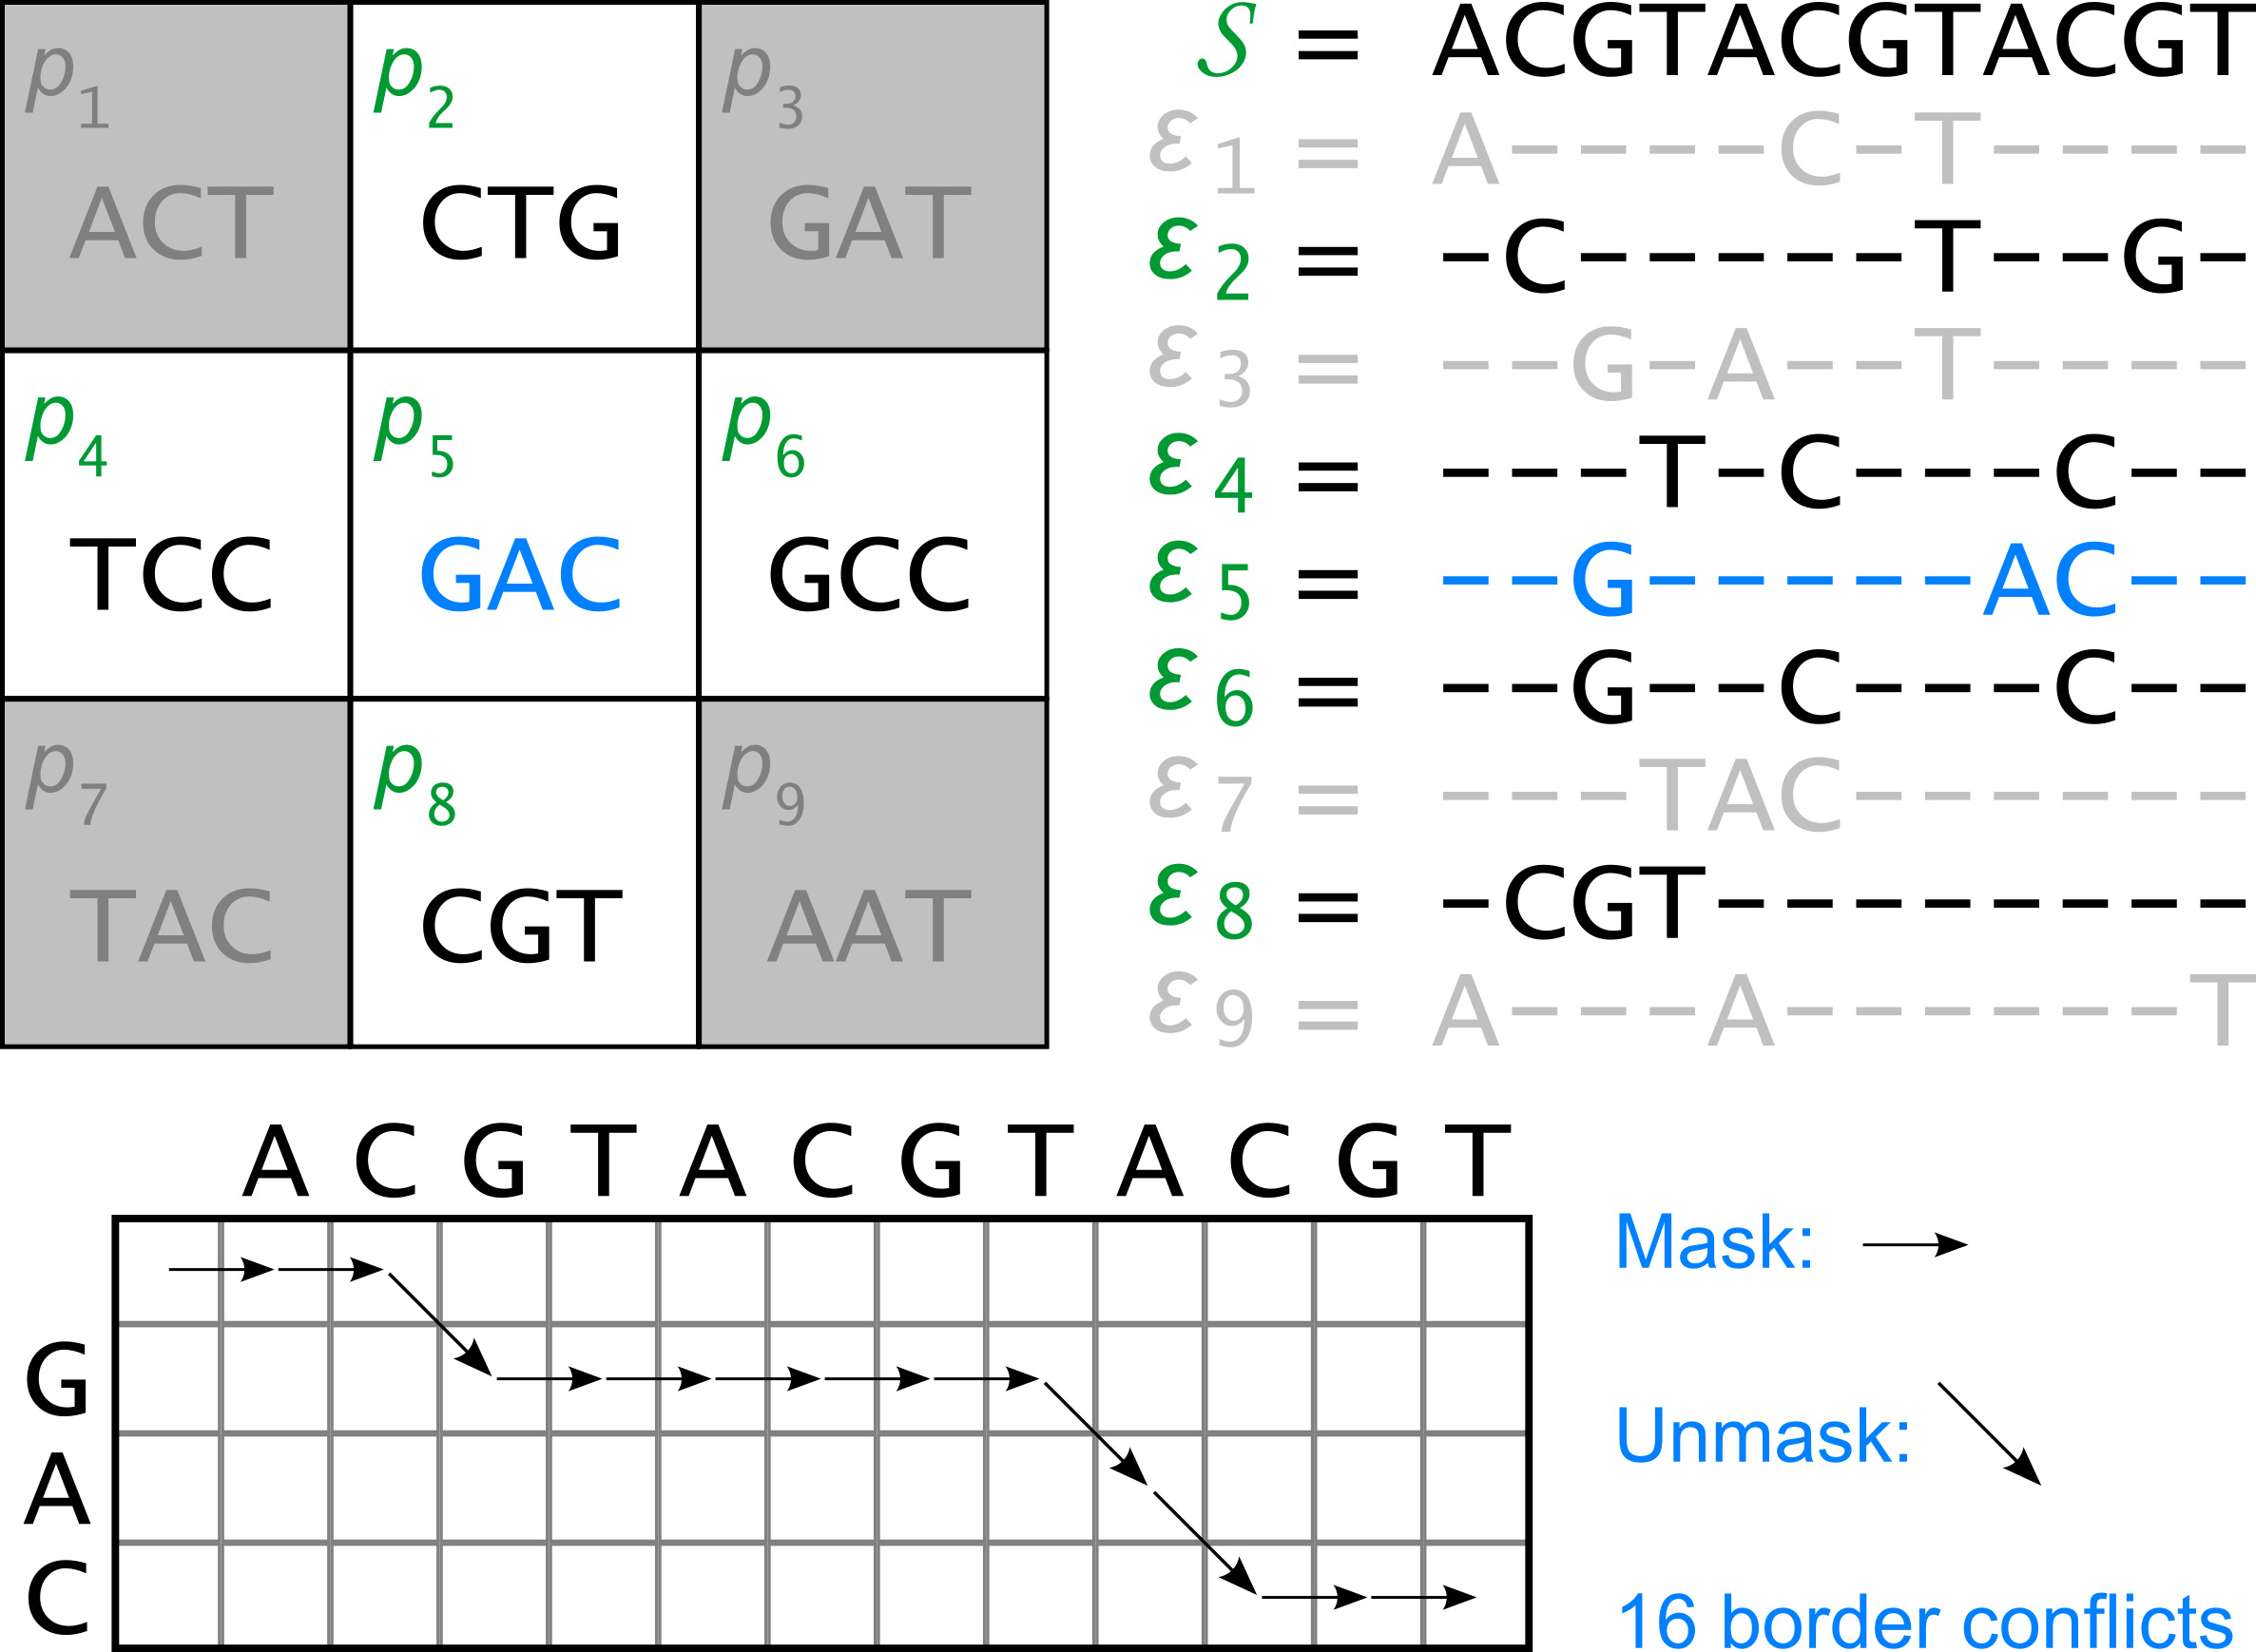
\includegraphics[width=0.8\textwidth]{pics/ospe2.jpg}}
  \end{overprint}

}

%%%%%%%%%%%%%%%%%%%%%%%%%%%%%%%%%%%%%%%%%%%%%%%%%%%%%%%%%%%%%%%%%%%%%%%%%%%%%%%%
\frame{\frametitle{Partitioning}

  The placement problem can be trivially \alert{partitioned}
  \begin{itemize}
    \item The chip is divided into sub-regions; each sub-region gets a sub-set
          of the probes
    \item Sub-regions are processed independently, and can be
          \alert{recursively partitioned}
    \item In the end, a placement algorithm is needed
    \item Can reduce run-time and help the placement algorithm
  \end{itemize}

  \begin{block}{Partitioning: Centroid Quadrisection (Kahng {\it et~al}., 2003)}
    \begin{itemize}
      \item The chip is divided into \alert{four quadrants}
      \item Four ``centroids'' are selected maximizing the Hamming distance 
            between their embeddings
      \item Remaining probes are compared to the centroids and are assigned to
            the quadrant whose centroid has the minimum Hamming distance
    \end{itemize}
  \end{block}

}

%%%%%%%%%%%%%%%%%%%%%%%%%%%%%%%%%%%%%%%%%%%%%%%%%%%%%%%%%%%%%%%%%%%%%%%%%%%%%%%%
\frame{\frametitle{Motivation}

  \begin{block}{Observation 1}
    \begin{itemize}
      \item The place and re-embed approach is inefficient
      \begin{itemize}
        \item Placement is based on embeddings that are likely to change
      \end{itemize}
    \end{itemize}
  \end{block}

  \begin{columns}
  
    \begin{column}{0.55\textwidth}
      \begin{block}{Observation 2}
        \begin{itemize}
          \item Some probes have only a few possible embeddings
          \item Others may have up to several millions
          \item Probes with more embeddings are more ``flexible''
          \begin{itemize}
            \item They can adapt better to their neighbors
          \end{itemize}
        \end{itemize}
      \end{block}
    \end{column}
    
    \begin{column}{0.45\textwidth}
      \centerline{\footnotesize{
      \begin{tabular}{|r|r|r|}
      \multicolumn{3}{c}{E.Coli GeneChip}     \\ \hline
         Number &       & Numer of            \\
      of probes &    \% & embeddings          \\ \hline
 \alert{1\,765} & \alert{0.78} & \alert{1}    \\
        28\,410	&  12.63       &           26 \\
        52\,913	&  23.52       &          351 \\
        63\,588	&  28.26       &       3\,276 \\
	48\,257	&  21.45       &      23\,751 \\
        22\,628	&  10.06       &     142\,506 \\
         6\,372	&   2.83       &     736\,281 \\
	    957	&   0.43       &  3\,365\,856 \\
             86	&   0.04       & 13\,884\,156 \\ \hline
       224\,976	& 100.00       &  	      \\ \hline
      \end{tabular}}}
    \end{column}
  
  \end{columns}
    
}

%%%%%%%%%%%%%%%%%%%%%%%%%%%%%%%%%%%%%%%%%%%%%%%%%%%%%%%%%%%%%%%%%%%%%%%%%%%%%%%%
\frame{\frametitle{Phase 1: Selecting Pivot Candidates}

  \begin{itemize}
    \item We use probes with fewer embeddings (\alert{pivots}) to:
    \begin{itemize}
      \item Drive the partitioning of the probe set
      \item Re-embed the probes before their placement
    \end{itemize}
  \end{itemize}
  
  \begin{block}{Algorithm 1: PivotPartitioning}
    \footnotesize{
    \begin{minipage}{\textwidth}
    
    \begin{tabbing}
    Output: \=                                  \kill
    Input:  \> chip dimensions,
               set of probes $\mathcal{P} = \{p_{1}, p_{2}, ... p_{n}\}$, and\\
            \> maximum partitioning depth $t_{max}$\\
    Output: \> placement of the probes $p \in \mathcal{P}$ on the chip
    \end{tabbing}
    
    \vspace*{-.5cm}
    
    \begin{itemize}
    \item[1.] Select probes $p$ with minimum number of embeddings, $E(p)$:
      \begin{itemize}\footnotesize{
      \item[a)] Let $\mathcal{Q} = \{p \in \mathcal{P} | E(p) \mbox{ is minimal}\}$
      \item[b)] $\mathcal{P} \leftarrow \mathcal{P} \setminus Q$
      }
      \end{itemize}
    \item[2.] Let $R$ be a region consisting of all spots
    \item[3.] Return RecursivePartitioning (1, $t_{max}$, $R$, $\mathcal{Q}$, $\mathcal{P}$)
    \end{itemize}
    \end{minipage}
    }
  \end{block}
  
}

%%%%%%%%%%%%%%%%%%%%%%%%%%%%%%%%%%%%%%%%%%%%%%%%%%%%%%%%%%%%%%%%%%%%%%%%%%%%%%%%
\frame{\frametitle{Phase 2: Recursive Partitioning}

  \begin{block}{Algorithm 2: RecursivePartitioning}
    \begin{minipage}{\textwidth}\footnotesize{
    
    \begin{tabbing}
    Output: \=                                  \kill
    Input:  \> current depth $t$, maximum depth $t_{max}$, region $R$,\\
            \> pivot candidates $\mathcal{Q}$, non-pivot probes $\mathcal{P}$,\\
    Output: \> placement of probes $p \in \mathcal{P} \cup \mathcal{Q}$ on $R$
    \end{tabbing}
    
    \vspace*{-.5cm}
    
    \begin{itemize}
    \item[1.] If $t = t_{max}$ then
      \begin{itemize}
        \item[a)] Re-embed $p \in \mathcal{P}$ optimally with respect to all $q \in \mathcal{Q}$
        \item[b)] Return RowEpitaxial ($R$, $\mathcal{P} \cup \mathcal{Q}$)
      \end{itemize}
    \item[2.] Select $q'$ and $q'' \in \mathcal{Q}$ with maximum conflicts $c(q',q'')$
    \item[3.] Partition $\mathcal{P}$ and $\mathcal{Q}$:
      \begin{itemize}
        \item[a)] Let $\mathcal{Q}' = \{q \in \mathcal{Q} \;|\; c(q,q') < c(q,q'')\}$;
                  $\mathcal{Q}'' \leftarrow \mathcal{Q} \setminus \mathcal{Q}'$
        \item[b)] Let $\mathcal{P}' = \{p \in \mathcal{P} \;|\; c(p,q') < c(p,q'')\}$;
                  $\mathcal{P}'' \leftarrow \mathcal{P} \setminus \mathcal{P}'$
      \end{itemize}
    \item[4.] Partition $R$ into $R'$ and $R''$ proportionally to
              $\mathcal{P}' \cup \mathcal{Q}' / \mathcal{P}'' \cup \mathcal{Q}''$
    \item[5.] Return RecursivePartitioning ($t + 1$, $t_{max}$, $R'$, $\mathcal{Q}'$, $\mathcal{P}$') \\
          $\cup$ RecursivePartitioning ($t + 1$, $t_{max}$, $R''$, $\mathcal{Q}''$, $\mathcal{P}$'')
    \end{itemize}
    
    }\end{minipage}
  \end{block}

}

%%%%%%%%%%%%%%%%%%%%%%%%%%%%%%%%%%%%%%%%%%%%%%%%%%%%%%%%%%%%%%%%%%%%%%%%%%%%%%%%
\frame{\frametitle{Remarks}

  Similar to the Centroid Quadrisection but...
  \begin{itemize}
    \item Alternate \alert{horizontal} and \alert{vertical} partitions
    \item Use probes with fewer embeddings as pivots (``centroids'')
    \begin{itemize}
      \item Faster selection, better representatives
    \end{itemize}
    \item First algorithm to combine \alert{placement} and \alert{embedding}
    \begin{itemize}
      \item Consider all embeddings when assigning probes to regions
      \item Re-embed probes optimally in regards to pivots (with OSPE) before
            the placement
    \end{itemize}
  \end{itemize}

}

%%%%%%%%%%%%%%%%%%%%%%%%%%%%%%%%%%%%%%%%%%%%%%%%%%%%%%%%%%%%%%%%%%%%%%%%%%%%%%%%
\frame{\frametitle{Results on Random Chips}

  \begin{block}{Border Length Minimization (cost: normalized border length)}
    \scriptsize{
    \centerline{
    \begin{tabular}{c|rr|rr|rr|rr}
& \multicolumn{2}{c|}{$t_{max}=0$} & \multicolumn{2}{c|}{$t_{max}=2$} & \multicolumn{2}{c|}{$t_{max}=4$} & \multicolumn{2}{c}{$t_{max}=6$} \\
Dim & \multicolumn{1}{c}{Cost} & \multicolumn{1}{c|}{Time} & \multicolumn{1}{c}{Cost} & \multicolumn{1}{c|}{Time} & \multicolumn{1}{c}{Cost} & \multicolumn{1}{c|}{Time} & \multicolumn{1}{c}{Cost} & \multicolumn{1}{c}{Time} \\
\noalign{\smallskip} \hline \noalign{\smallskip}
100 & 42.77 &     34 & 39.19 &     13 & 40.72 &     10 & 42.11 &  11 \\
200 & 41.63 &    429 & 37.30 &    155 & 38.53 &     62 & 40.00 &  85 \\
300 & 41.38 & 1\,174 & 36.12 &    766 & 37.22 &    264 & 38.53 & 139 \\
500 & 41.27 & 3\,524 & 34.69 & 3\,472 & 35.50 & 1\,996 & 36.58 & 713 \\
    \noalign{\smallskip}
    \end{tabular}}
    }
  \end{block}

  \begin{block}{Conflict Index minimization (cost: average conflict index)}
    \scriptsize{
    \centerline{
    \begin{tabular}{c|rr|rr|rr|rr}
& \multicolumn{2}{c|}{$t_{max}=0$} & \multicolumn{2}{c|}{$t_{max}=2$} & \multicolumn{2}{c|}{$t_{max}=4$} & \multicolumn{2}{c}{$t_{max}=6$} \\
Dim & \multicolumn{1}{c}{Cost} & \multicolumn{1}{c|}{Time} & \multicolumn{1}{c}{Cost} & \multicolumn{1}{c|}{Time} & \multicolumn{1}{c}{Cost} & \multicolumn{1}{c|}{Time} & \multicolumn{1}{c}{Cost} & \multicolumn{1}{c}{Time} \\
\noalign{\smallskip} \hline \noalign{\smallskip}
100 & 514.49 &     45 & 453.67 &     37 & 467.78 &     19 & 475.44 &     15 \\
200 & 517.07 &    192 & 466.22 &    215 & 452.41 &    166 & 462.55 &     99 \\
300 & 518.51 &    438 & 475.84 &    524 & 452.00 &    466 & 448.17 &    336 \\
500 & 517.50 & 1\,471 & 481.36 & 1\,530 & 462.33 & 1\,472 & 445.43 & 1\,295 \\
    \noalign{\smallskip}
    \end{tabular}}
    }
  \end{block}

  \ignore{
  \scriptsize{
    Row-epitaxial is used for the placement (with $Q = 20\,000$), followed by
    Sequential re-embedding; running times reported in seconds.
  }
  }
}

%%%%%%%%%%%%%%%%%%%%%%%%%%%%%%%%%%%%%%%%%%%%%%%%%%%%%%%%%%%%%%%%%%%%%%%%%%%%%%%%
\frame{\frametitle{Pivot Partitioning (PP) $\times$ Centroid Quadrisection (CQ)}

  \begin{block}{Border Length Minimization}
    \scriptsize{
    \centerline{
    \begin{tabular}{c|rr|rr|rr}
& \multicolumn{1}{|c}{$L=1$} & \multicolumn{1}{c}{$t_{max}=2$} & \multicolumn{1}{|c}{$L=2$} & \multicolumn{1}{c}{$t_{max}=4$} & \multicolumn{1}{|c}{$L=3$} & \multicolumn{1}{c}{$t_{max}=6$} \\
Dim & \multicolumn{1}{|c}{CQ} & \multicolumn{1}{c}{PP} & \multicolumn{1}{|c}{CQ} & \multicolumn{1}{c}{PP} & \multicolumn{1}{|c}{CQ} & \multicolumn{1}{c}{PP} \\
\noalign{\smallskip} \hline \noalign{\smallskip}
100 &    393\,218 & 0.18\% &    399\,312 & -1.89\% &    410\,608 & -2.48\% \\
200 & 1\,524\,803 & 2.27\% & 1\,545\,825 &  0.48\% & 1\,573\,096 & -1.34\% \\
300 & 3\,493\,552 & 7.12\% & 3\,413\,316 &  2.05\% & 3\,434\,964 & -0.61\% \\
500 & 9\,546\,351 & 8.95\% & 9\,355\,231 &  4.67\% & 9\,307\,510 &  1.03\% \\
    \noalign{\smallskip}
    \end{tabular}}
    }
  \end{block}

}

%% *****************************************************************************
\section*{Summary}
\subsection*{Dummy}
%% *****************************************************************************

%%%%%%%%%%%%%%%%%%%%%%%%%%%%%%%%%%%%%%%%%%%%%%%%%%%%%%%%%%%%%%%%%%%%%%%%%%%%%%%%
\frame{\frametitle{Summary}

  \begin{itemize}
    \item \alert{Conflict Index}: new model for evaluating microarray layouts
    \item \alert{Pivot Partitioning}: new partitioning algorithm
    \begin{itemize}
      \item Faster and better selection of pivots
      \item Improved assignment of probes to regions
      \item First to combine placement and re-embedding
    \end{itemize}
    
    \vskip0pt plus.5fill

    \ignore{    
    \item Future work
    \begin{itemize}
      \item Implement ``borrowing heuristic''
    \end{itemize}
    }
    
  \end{itemize}

}

%%%%%%%%%%%%%%%%%%%%%%%%%%%%%%%%%%%%%%%%%%%%%%%%%%%%%%%%%%%%%%%%%%%%%%%%%%%%%%%%
\begin{frame}{Thanks!}

  \centerline{
    
\includegraphics[height=1.4cm]{pics/aggi_logo.png}
    \hspace*{0.6cm}
    
\includegraphics[height=1.4cm]{pics/gsbg_logo.png}
  }

  \begin{itemize}
    \item Prof. Dr. Jens Stoye
    \item Prof. Dr. Robert Giegerich
    \item AG Genominformatik
    \item Graduiertenkolleg Bioinformatik
    \item Graduate School in Bioinformatics and Genome Research
    
    \vskip0pt plus.5fill
    
    \item ...and \alert{thank you} for your attention!
    
  \end{itemize}
  
  \begin{block}{More info on}
    \centerline{\tt\alert{
      http://gi.cebitec.uni-bielefeld.de/assb/chiplayout
    }}
  \end{block}
  
\end{frame}

\end{document}
